%!TEX root = ../risk_report.tex

\chapter{Findings} \label{chap:findings}

\noindent Findings are organised according to the formulation of areas of interest as questions. These questions progress from general frequency counting (Q1), through experiential meanings (Qs 2--7), to risk as modifier (Qs 8 \& 9) and finally to arguability (Q10). Discussion of the general significance of individual findings is also presented in this section, as the Discussion section synergises all findings to explain the discourse-semantics of risk.

An \emph{IPython Notebook} interface for navigating the corpus \cite<see>{mckinney_python_2012}, as well as the code used to interrogate it and the findings we produced, is available online: \url{https://github.com/interrogator/risk}. A non-interactive version is available at \url{http://nbviewer.ipython.org/github/interrogator/risk/blob/master/risk.ipynb}. This Notebook does not suffer from spatial limitations, and thus contains additional information, including the exact Tregex queries used in interrogations, as well as complete lists of the concordance lines discussed only briefly here. Tools and results from other kinds of corpus linguistic analysis, such as keywording and collocation, are also available there, but have not been described here.

\section{How frequently do risk words appear?} 
\FloatBarrier

	%We successfully located a number of lexicogrammatical sites of change within clauses containing a risk word. 

	The first point of interest was the overall frequency of risk words in the NYT (Figure \ref{fig:relative_frequency_of_risk_words}) and the distribution of risk words by word class (nominal, verbal, adjectival\slash adverbial), absent any consideration of surrounding grammar (see Figure \ref{fig:wordclasses}). In terms of the relative frequency of risk words, we note a general upward trend, with a number of peaks and troughs worthy of further investigation. In terms of word classes of risk, we found that not only are nominal forms by far the most common in the NYT, but that it is nominal risk words that vary the most in frequency, with the other categories remaining more or less stable. Interestingly, in the span for which we have no data (1964--1986), adjectival forms overtake verbal forms of risk in frequency.

    %Using our reference corpus, we checked to see whether nominals were becoming more frequent within the NYT more generally.
          \noindent
          \begin{figure}[htb!]
          \centering
          \begin{minipage}{.45\textwidth}
            \centering
                      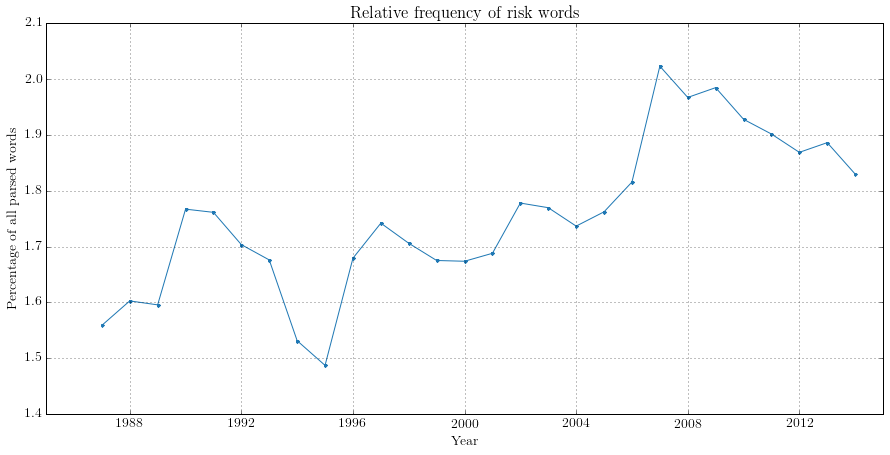
\includegraphics[width=.95\textwidth]{../images/relative_frequency_of_risk_words.png}
                      \caption{Relative frequency of risk words}
                      \label{fig:relative_frequency_of_risk_words}
          \end{minipage}%
          \begin{minipage}{.55\textwidth}
            \centering
                      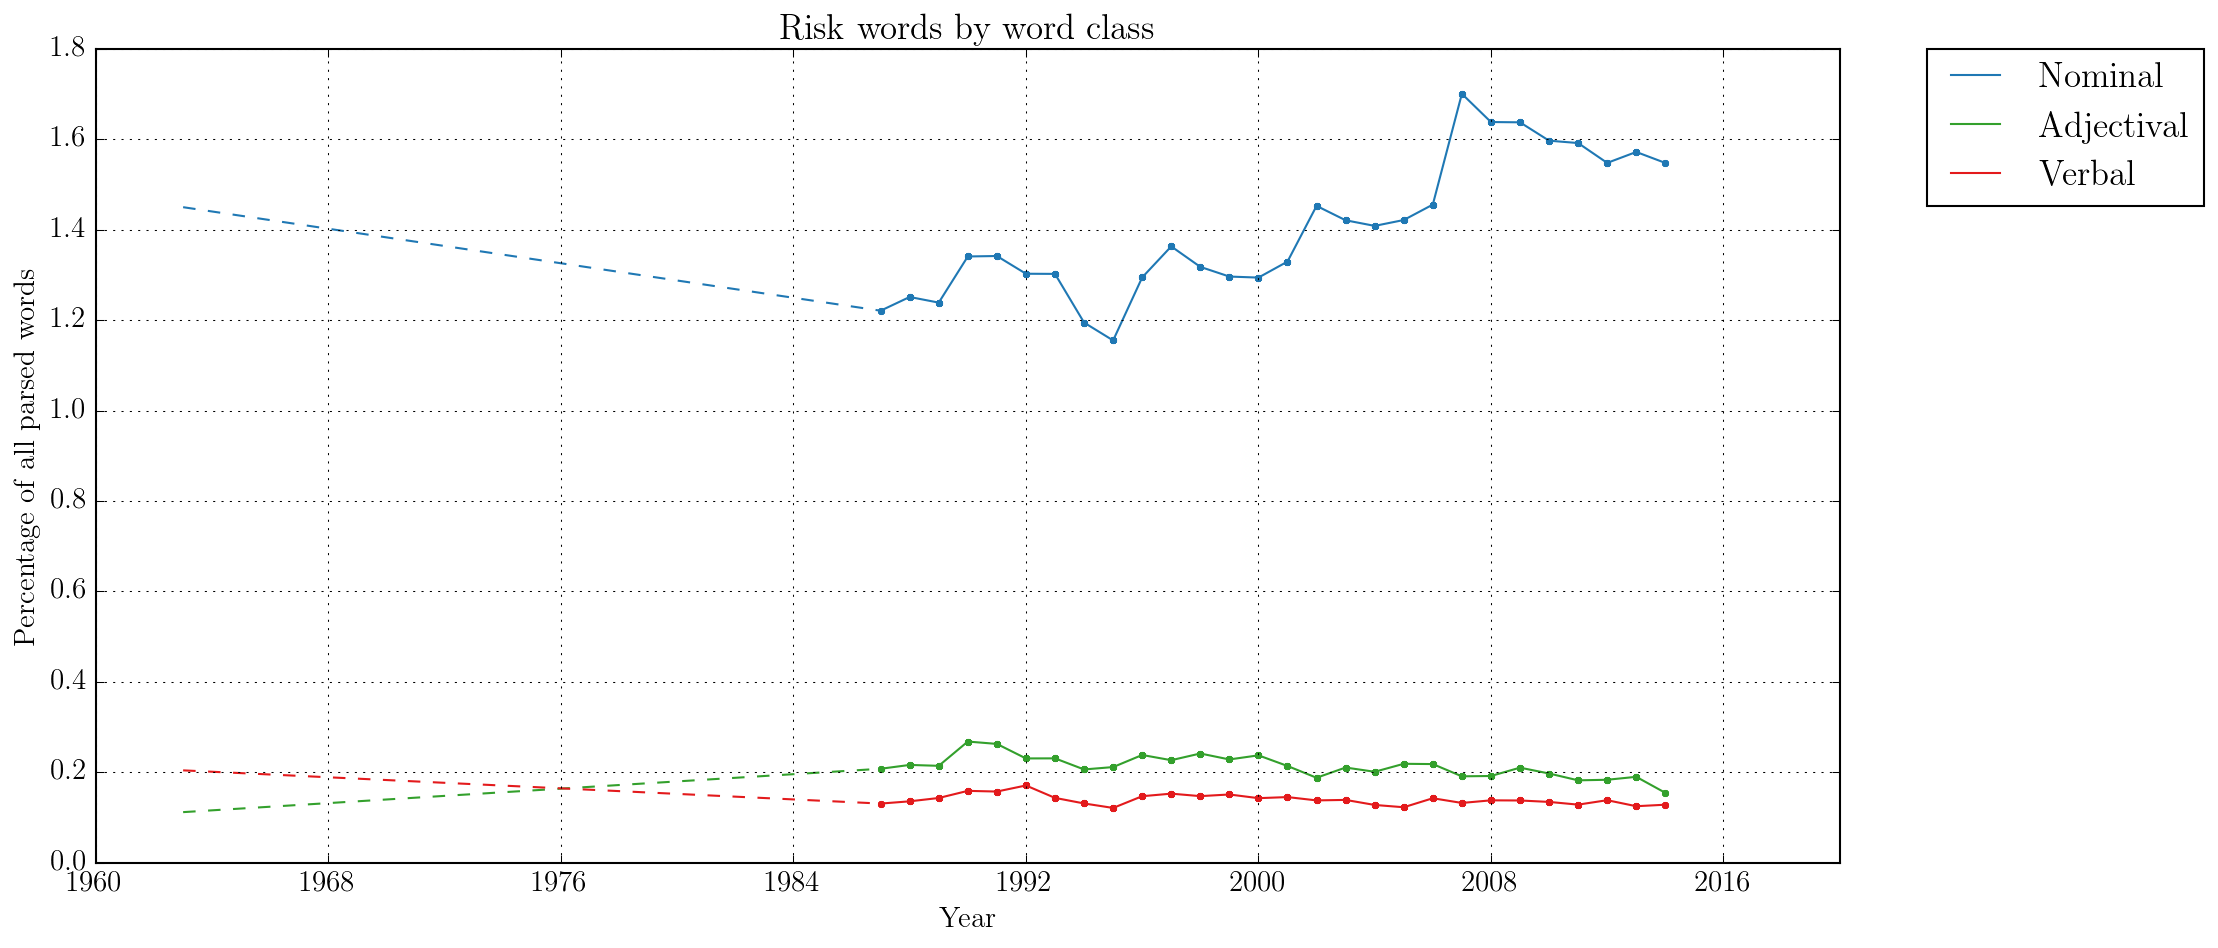
\includegraphics[width=.95\textwidth]{../images/risk_words_by_word_class.png}
                      \caption{Relative frequency by word class}
                      \label{fig:wordclasses}
          \end{minipage}
          \end{figure}



			%\begin{figure}[htb!]
			%\centering
			%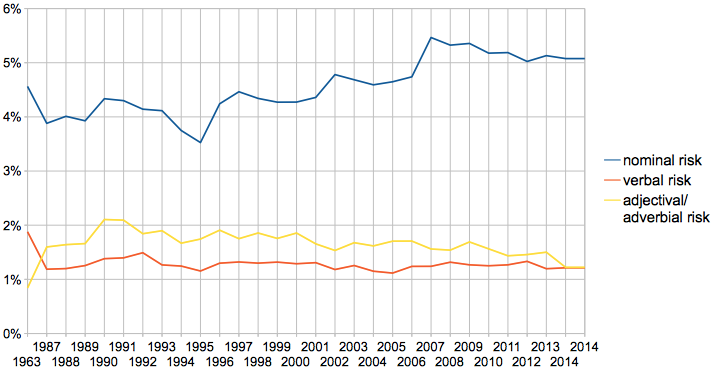
\includegraphics[width=0.75\textwidth]{../images/relwordclass.png}
			%\caption{Risk words by word class as percentage of all parsed words}
			%\label{fig:relwordclass}
			%\end{figure}

			%FUNCTIONAL CATEGORISATION?

	We compared this against the relative frequencies of nominal, verbal and adjectival/adverbial lexical items in the corpus as a whole, in order to account for any trends toward nominalisation in our dataset more generally (Figure \ref{fig:wordclasses}). This showed that even when compared to potential trends toward nominalisation generally, nominal risks are still on an inbound trajectory.


	These initial findings guided the rest of the investigation: particular attention was paid to nominal risks, as these were the site of the most longitudinal change. That said, these categories provide merely a categorisation of the formal features of risk words. Functionally, things are substantially more complicated: \emph{running a risk}, for example, while featuring a nominal risk, is in reality a risk process; similarly, though risk is nominal in \emph{risk management}, risk is nominal, it functions as a modifier, rather than a participant.

    A similar question is the number of unique risk words appearing per year. Figure \ref{fig:diffriskwords} demonstrates that there does appear to be a general increase in the relative number of risk words over time. That said, given that approximately half of unique tokens in each subcorpus appear only once, 
        1963 is excluded from analysis here, as poor quality OCR created a number of non-word results.

            \begin{figure}[htb!]
            \centering
            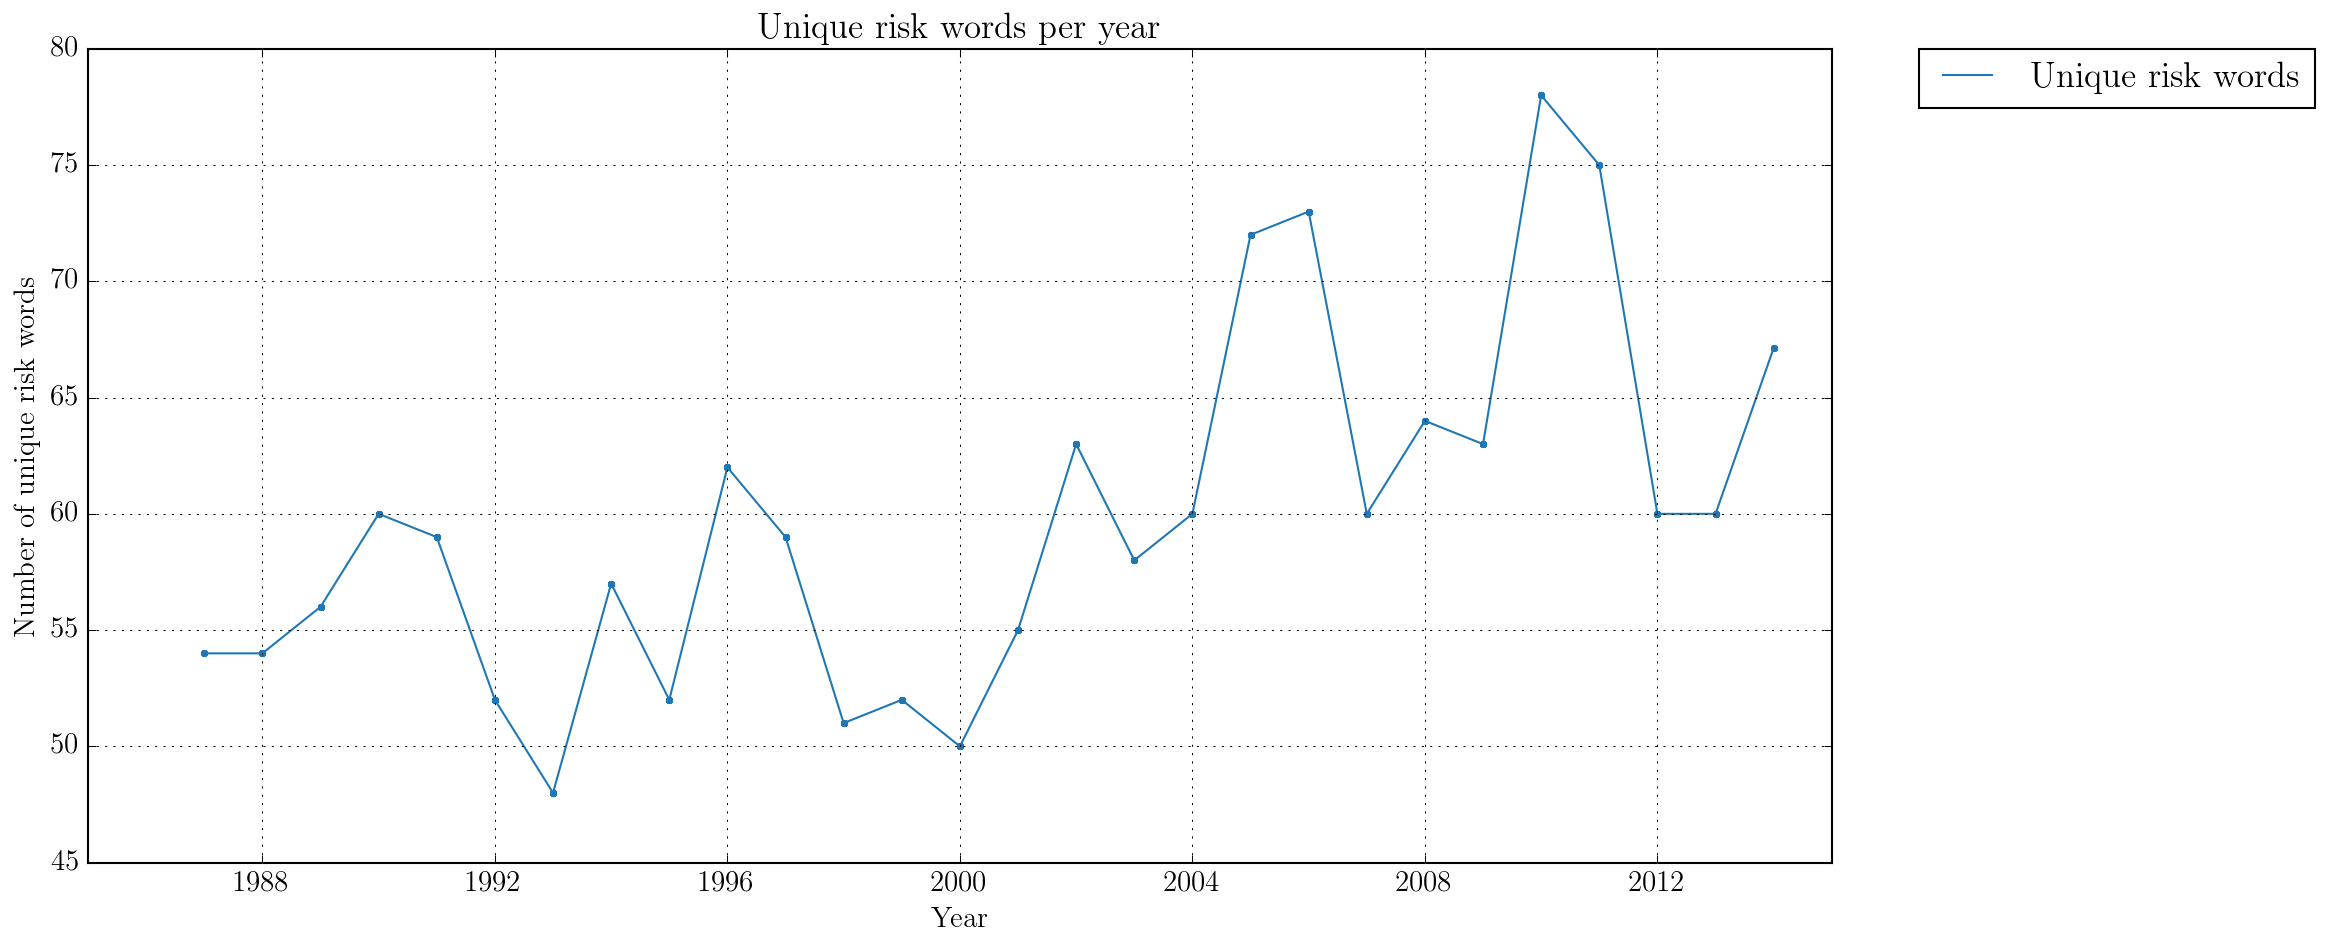
\includegraphics[width=0.7\textwidth]{../images/unique_risk_words_per_year.png}
            \caption{Unique risk words}
            \label{fig:diffriskwords}
            \end{figure}


	%\section{Experiential meaning: risk as Participant and Process}

	\section{Which experiential roles do risk words occupy?} 
	\FloatBarrier

	Within the Transitivity system, a risk word may take the form of a participant (\emph{The risk was there}), process (\emph{I risked it}) or a modifier (\emph{a risky encounter}). Using both constituency parsing\slash SFL categories and Stanford CoreNLP's dependency parsing, we counted the frequency of risk words within these three functional roles (Figure \ref{fig:funcrole}). In line with the results from word-class based searching, we find that risk as a process is declining in use. Risk as modifier, patterning with adjectival risk, today comprises a larger proportion of risk participants than in earlier samples.
    %Somewhat unexpectedly, the results were very similar to the word-class based results.

		  \noindent
          \begin{figure}[htb!]
          \centering
          \begin{minipage}{.48\textwidth}
			\centering
			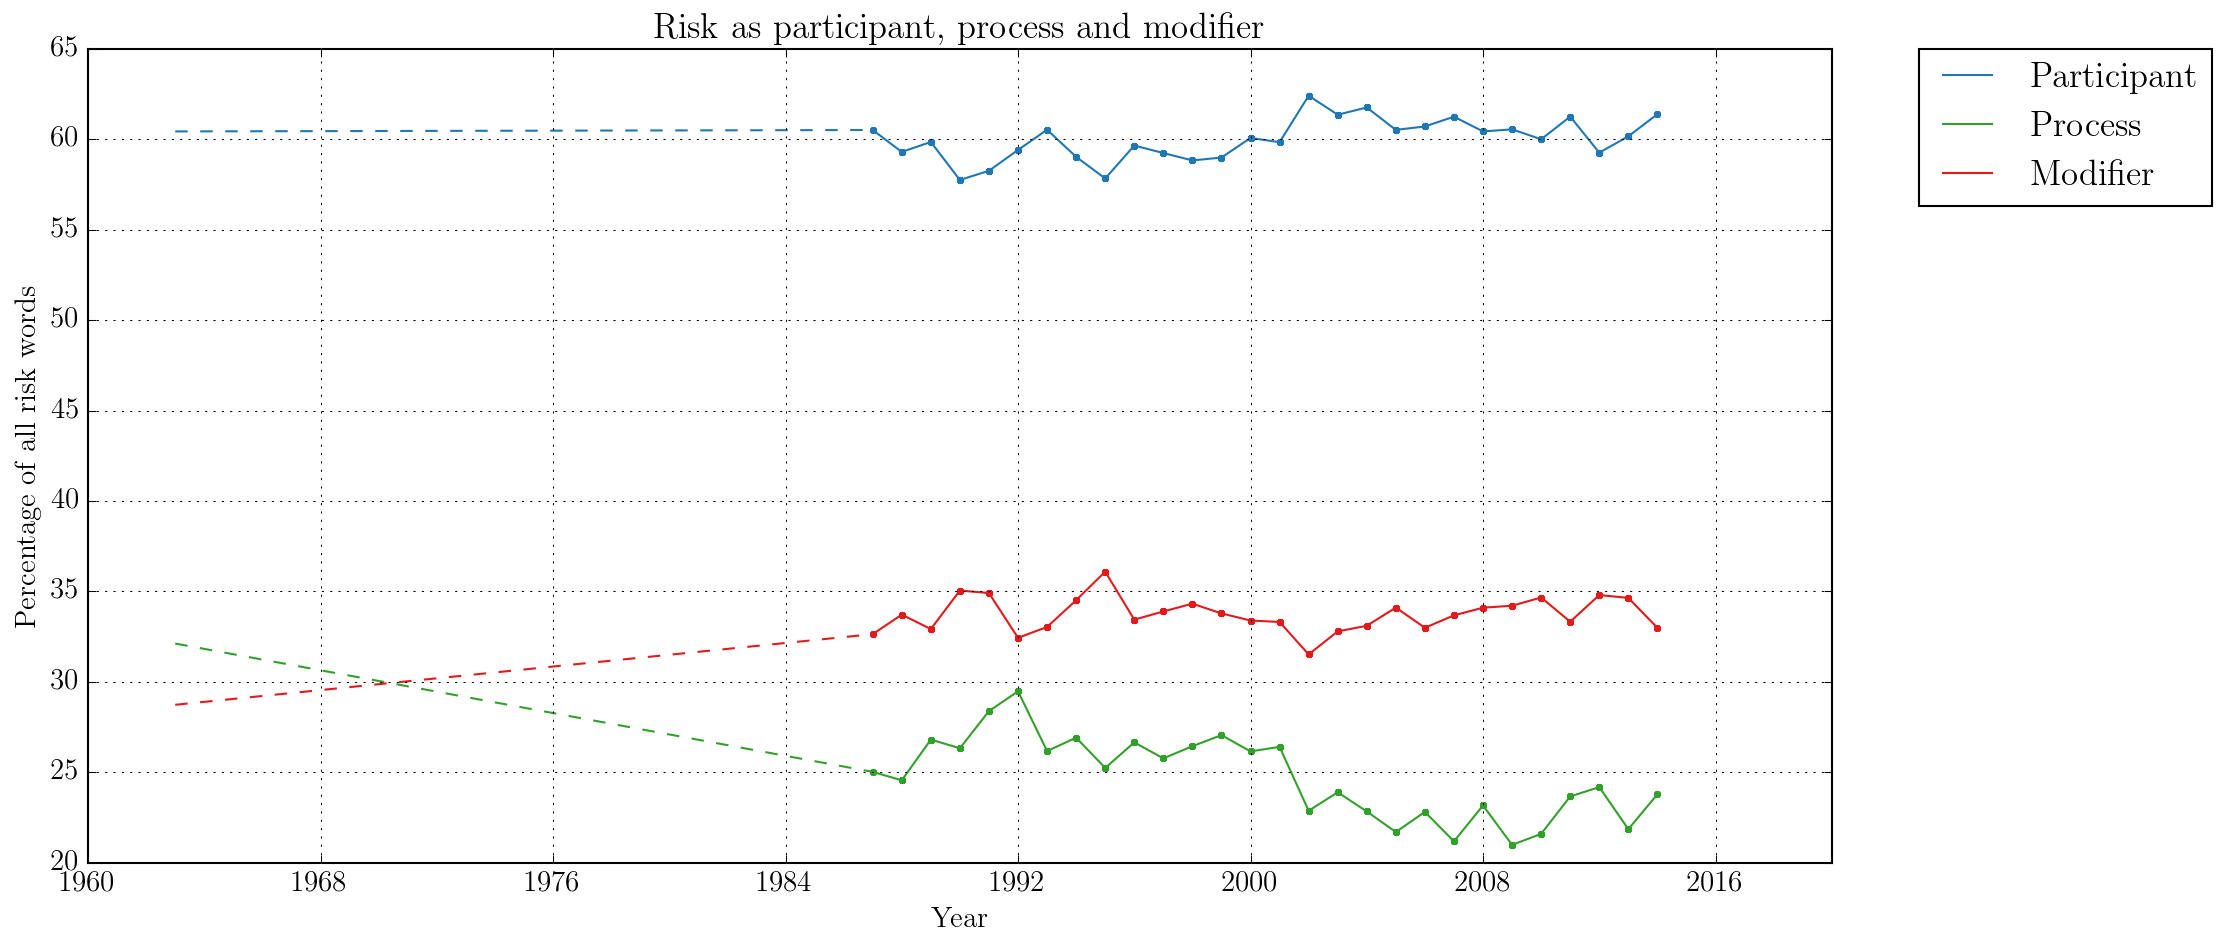
\includegraphics[width=0.98\textwidth]{../images/risk_as_participant,_process_and_modifier.png}
          \end{minipage}%
          \begin{minipage}{.48\textwidth}
            \centering
            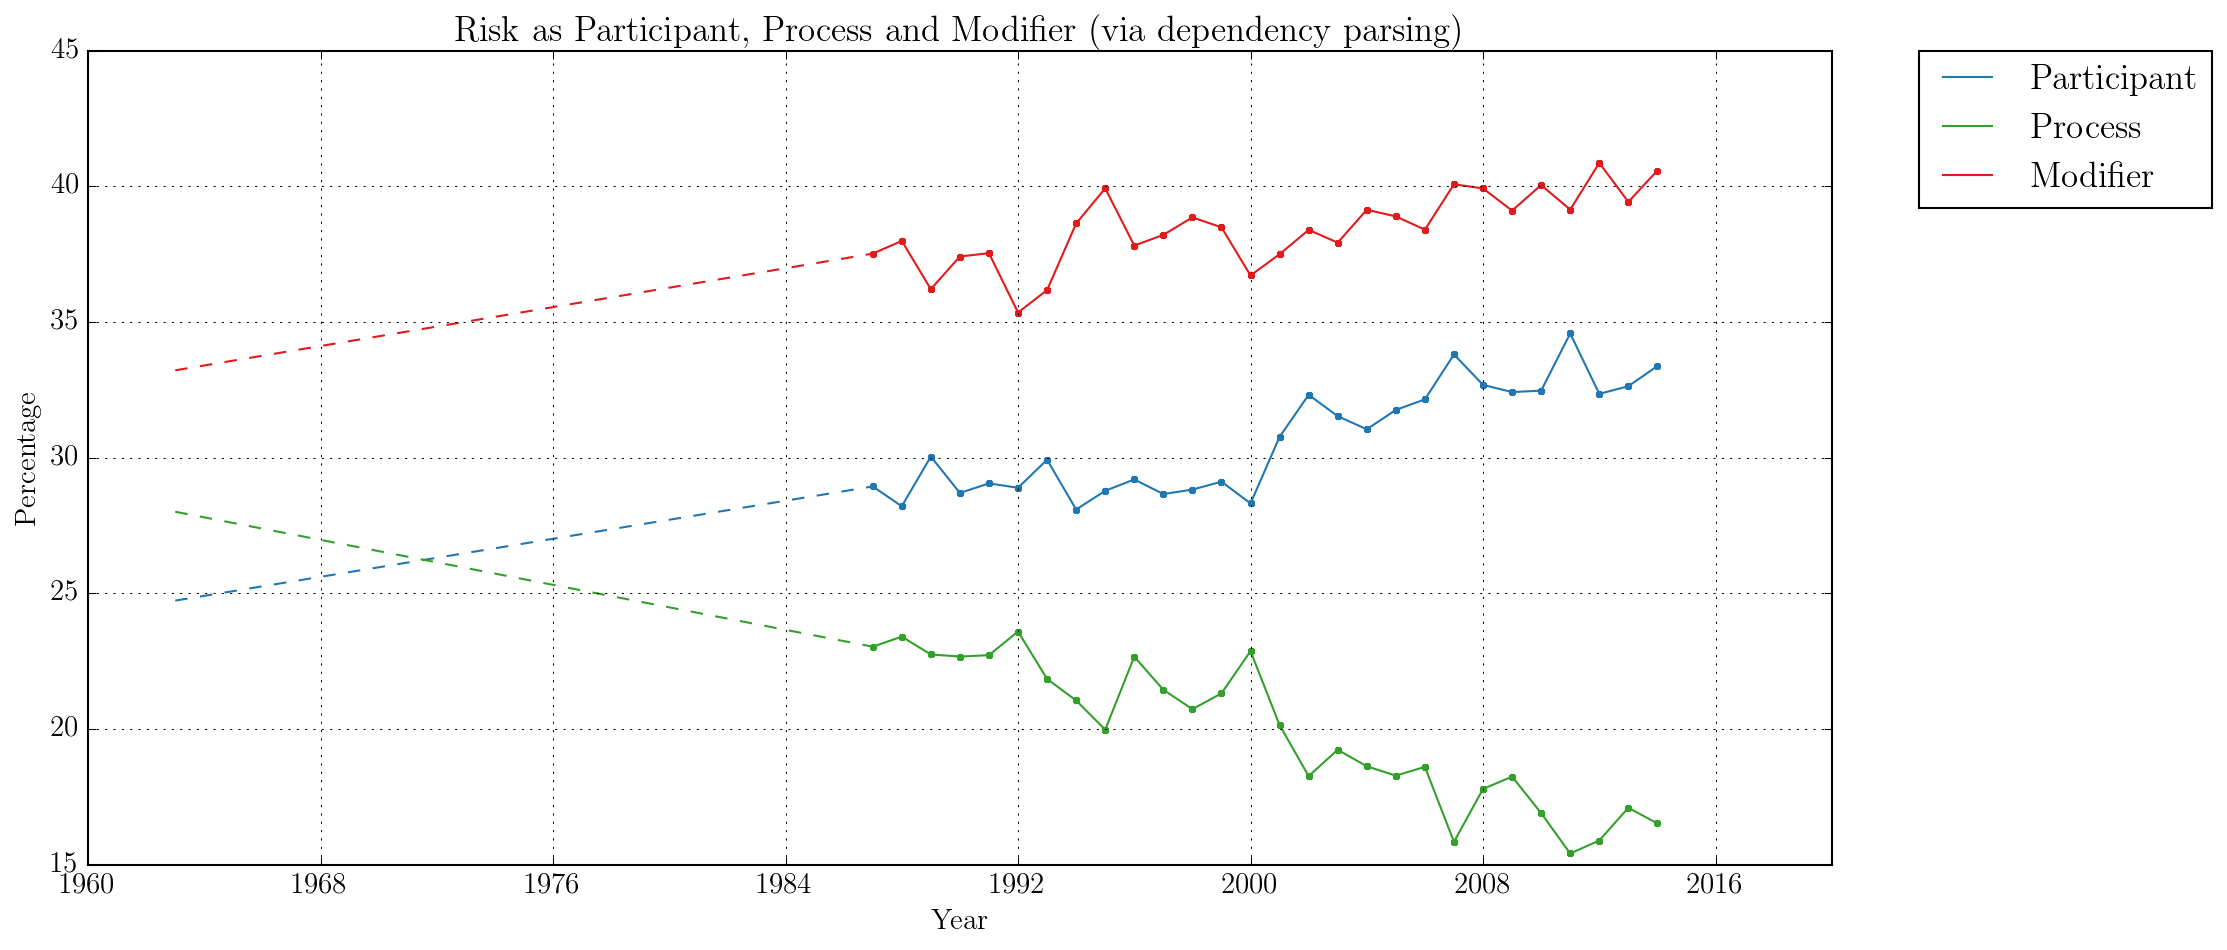
\includegraphics[width=0.98\textwidth]{../images/risk-as-participant-process-and-modifier-via-dependency-parsing.png}
           \end{minipage}
           \caption{Functional roles of risk words (via constituency and dependency parses)}
                \label{fig:funcrole}
          \end{figure}

	%~\ \todo[inline,color=green!40]{\noindent More discussion here, perhaps, as well as the above chart as relative frequencies. I may also have to account for risk within prepositional phrases here.}
		
	%only when the risk word forms the head of these groups, rather than a dependent/modifier (e.g. \emph{a risky decision}).

		\section{Is risk more commonly in the position of experiential subject or experiential object?} 
		\FloatBarrier

		Risk as a participant may take the form of an experiential subject or an experiential object. Our first area of interest was the proportion of each, with respect to general trends in the NYT. As shown in Figure \ref{fig:bestexpsubjobj}, risk is more commonly an object than a subject. It is also apparent that risk as experiential subject is on an static trajectory, while risk as experiential object is inbound. The significance of this is discussed in more depth in Section \ref{sect:arguability}.

			\begin{figure}[htb!]
			\centering
			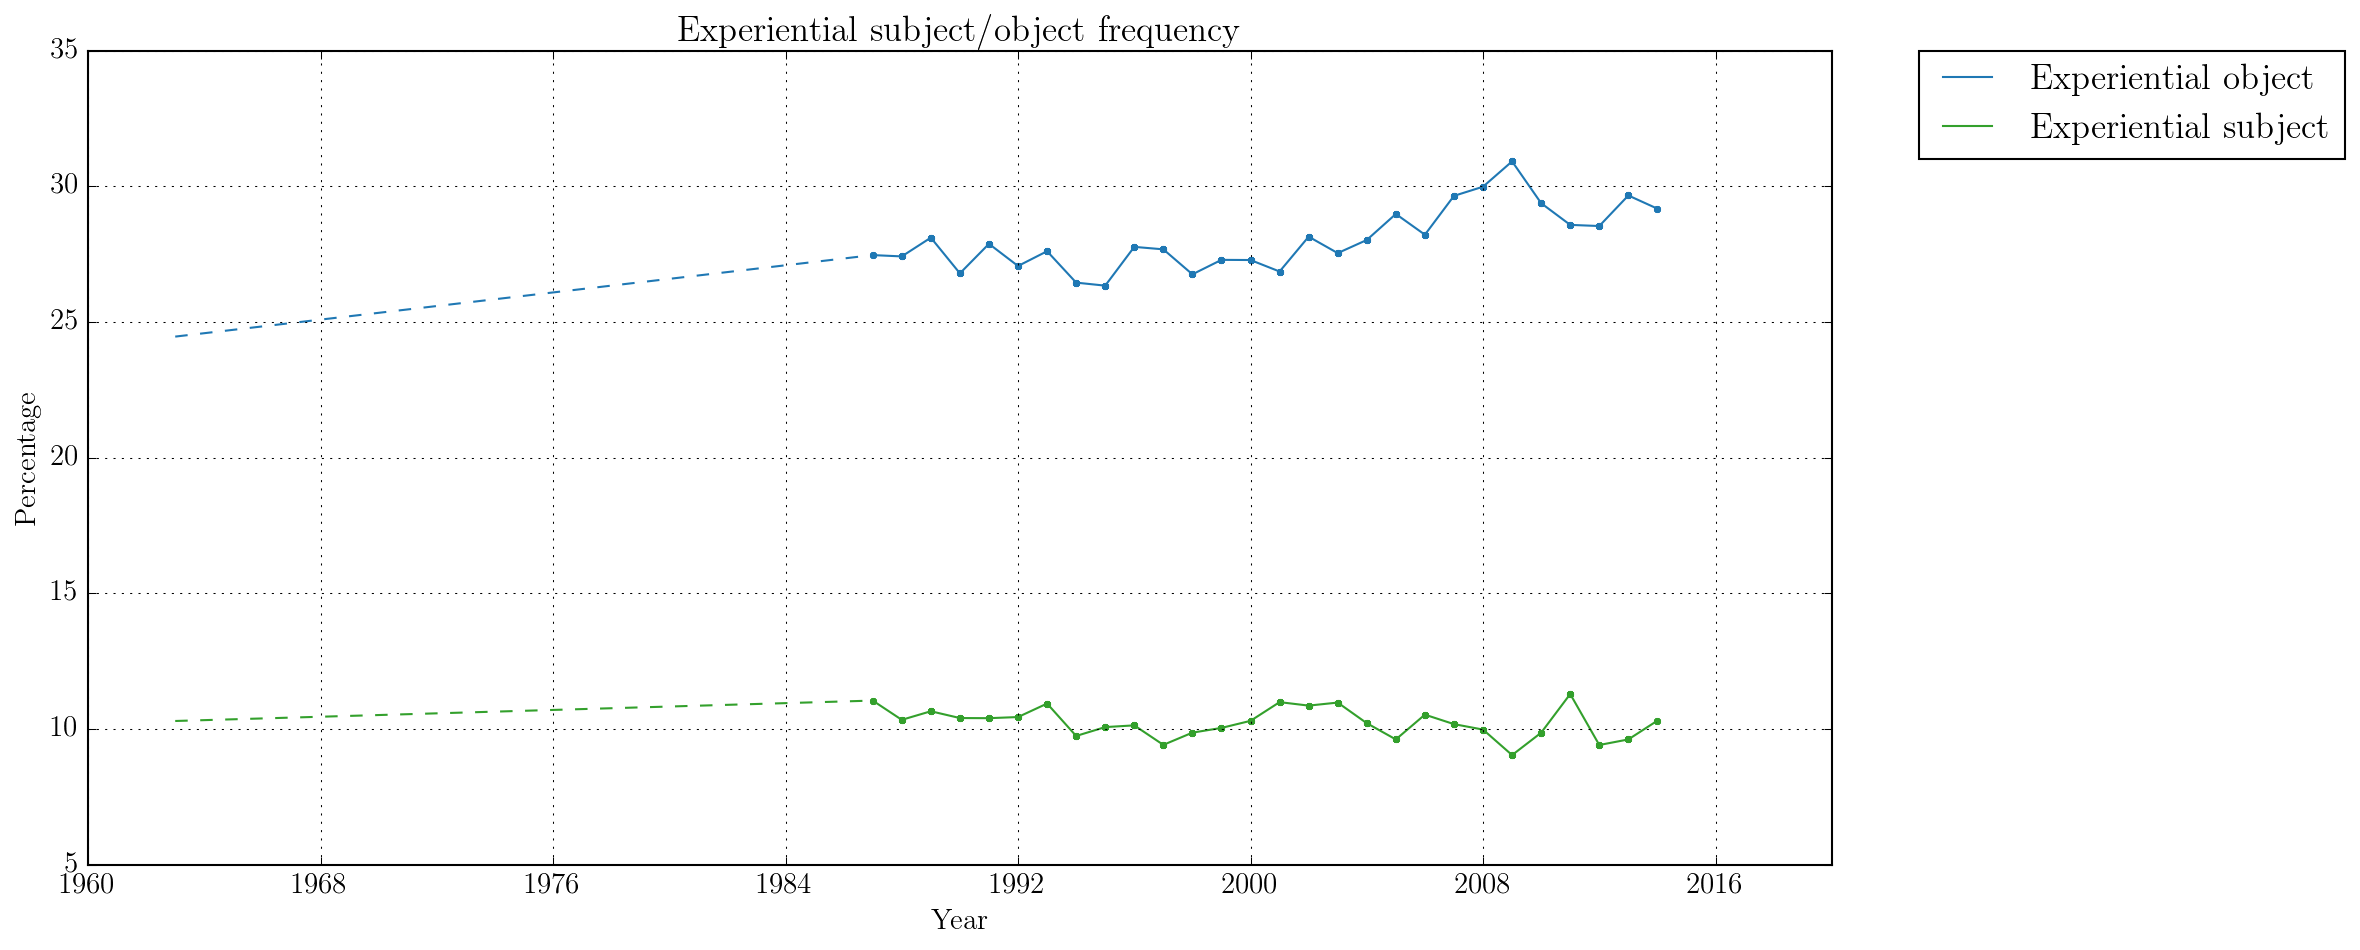
\includegraphics[width=0.75\textwidth]{../images/experiential_subject_object_frequency.png}
			\caption{Risk as experiential subject and object as percentage of all risk roles}
			\label{fig:bestexpsubjobj}
			\end{figure}
			%

    \begin{table}[tb]\footnotesize
    \centering
    \addvbuffer[12pt 8pt]{\begin{tabularx}{0.75\textwidth}{|X|X|}
    \hline
    \textbf{As subject} & \textbf{As object} \\ \hline
    \textit{But the most prevalent \textbf{risk} for the average traveler to Peru is the high altitude of the Andes}   & \textit{The company has resolved accounting problems, he said, and stabilized profit margins, while new management has reduced the company's \textbf{risks}}  \\ \hline
    \textit{The \textbf{risk} would be that the stock would recover during the period that the investor was out of the stock}   & \textit{But an empty village is a big \textbf{risk}.}  \\ \hline
    \textit{But the \textbf{risk}, though very small, that a man facing execution could win a new trial raises the question why this rule has proved so hard to follow}   & \textit{They said there was only a little \textbf{risk}, and now he 's not with us anymore} \\ \hline
    \end{tabularx}}
    \caption{Examples of risk as experiential subject and object in 2001}
    \label{tab:subj_conc}
    \end{table}

	\section{What processes are involved when risk is a participant?}
	\FloatBarrier

		We then wanted to determine the most common processes in which risk as a participant is involved. Tables \ref{tab:subj} and \ref{tab:obj} show the top twenty processes for risk as experiential subject and object, taking passivisation into account.\endnote{\emph{Take} and \emph{run} are removed from the object column here, as \emph{take risk} and \emph{run risk} are considered risk processes.}~

			% this below doesn't count agent as an experiential subject, and it should! also copula

					\begin{table}[htb!]
					\centering
										\addvbuffer[12pt 8pt]{\begin{minipage}{.35\textwidth}
										\small
										\begin{tabularx}{1.0\textwidth}{|>{\raggedright}X|l|}
										\hline
										\textbf{Processes when risk is experiential subject} & \textbf{Total} \\ \hline
										be                                      & 8954  \\ \hline
										increase                                & 460   \\ \hline
										outweigh                                & 278   \\ \hline
										rise                                    & 269   \\ \hline
										say                                     & 222   \\ \hline
										come                                    & 201   \\ \hline
										remain                                  & 192   \\ \hline
										go                                      & 190   \\ \hline
										have                                    & 179   \\ \hline
										make                                    & 148   \\ \hline
										seem                                    & 148   \\ \hline
										involve                                 & 145   \\ \hline
										grow                                    & 133   \\ \hline
										exist                                   & 127   \\ \hline
										take                                    & 121   \\ \hline
										become                                  & 120   \\ \hline
										lose                                    & 120   \\ \hline
										include                                 & 113   \\ \hline
										appear                                  & 111   \\ \hline
										pay                                  & 100   \\ \hline
										\end{tabularx}
										\caption{Processes when risk is \mbox{experiential} subject}
										\label{tab:subj}
										\end{minipage}} \hspace{1cm} % This must go next to `\end{minipage}`
										\addvbuffer[12pt 8pt]{\begin{minipage}{.35\textwidth}
										\small
										\begin{tabularx}{1.0\textwidth}{|>{\raggedright}X|l|}
										\hline
										\textbf{Processes when risk is experiential object} & \textbf{Total} \\ \hline
										%take                                             & 11459 \\ \hline
										reduce                                           & 5609  \\ \hline
										pose                                             & 4179  \\ \hline
										increase                                         & 4063  \\ \hline
										%run                                              & 3506  \\ \hline
										have                                             & 2879  \\ \hline
										carry                                            & 2115  \\ \hline
										face                                             & 1477  \\ \hline
										raise                                            & 1115  \\ \hline
										minimize                                         & 1009  \\ \hline
										assess                                           & 841   \\ \hline
										create                                           & 731   \\ \hline
										outweigh                                         & 704   \\ \hline
										avoid                                            & 683   \\ \hline
										present                                          & 619   \\ \hline
										assume                                           & 593   \\ \hline
										consider                                         & 588   \\ \hline
										see                                              & 563   \\ \hline
										understand                                       & 493   \\ \hline
										accept                                           & 492   \\ \hline
										weigh & 473   \\ \hline
										eliminate & 450   \\ \hline
			
										\end{tabularx}
										\caption{Processes when risk is experiential object}
										\label{tab:obj}
										\end{minipage}}
										\end{table}


	\section{How are participant risks modified?}
	\FloatBarrier

				Most commonly, risk as a participant is modified through adjectival pre-head modification or post-head modification with a subordinate clause or prepositional phrase. Ignoring the distinction between subject and object risk, and collapsing pre-head and post-head kinds of modification, Tables \ref{tab:prehead} and \ref{tab:posthead} show the most common pre- and post-head modifiers of risk as a participant.

					\begin{table}%[htb!]
					\centering
					\addvbuffer[12pt 8pt]{\begin{minipage}{0.35\textwidth}
					\raggedleft
					\small
					\begin{tabular}{|l|l|}
					\hline
					\textbf{Pre-head modifier}     & \textbf{Total} \\ \hline
					high         & 4753  \\ \hline
					great        & 3444  \\ \hline
					big          & 1672  \\ \hline
					political    & 1520  \\ \hline
					potential    & 1340  \\ \hline
					financial    & 1164  \\ \hline
					low          & 1056  \\ \hline
					more         & 1051  \\ \hline
					significant  & 1003  \\ \hline
					serious      & 935   \\ \hline
					real         & 869   \\ \hline
					little       & 761   \\ \hline
					own          & 713   \\ \hline
					substantial  & 547   \\ \hline
					less         & 541   \\ \hline
					such         & 514   \\ \hline
					calculated   & 469   \\ \hline
					considerable & 463   \\ \hline
					possible     & 458   \\ \hline
					other        & 423   \\ \hline
					\end{tabular}
					\caption{Pre-head modification of participant risk}
					\label{tab:prehead}
					\end{minipage}} \hspace{1cm}% This must go next to `\end{minipage}`
					\addvbuffer[12pt 8pt]{\begin{minipage}{0.35\textwidth}
						\raggedright
					\small
					\begin{tabular}{|l|l|}
					\hline
					\textbf{Post-head modifier} & \textbf{Total} \\ \hline
					cancer             & 2344  \\ \hline
					disease            & 1777  \\ \hline
					attack             & 1597  \\ \hline
					death              & 1025  \\ \hline
					injury             & 823   \\ \hline
					infection          & 811   \\ \hline
					loss               & 408   \\ \hline
					war                & 391   \\ \hline
					failure            & 383   \\ \hline
					inflation          & 368   \\ \hline
					problem            & 346   \\ \hline
					default            & 336   \\ \hline
					stroke             & 325   \\ \hline
					complication       & 288   \\ \hline
					damage             & 251   \\ \hline
					transmission       & 248   \\ \hline
					harm               & 244   \\ \hline
					aid                & 227   \\ \hline
					recession          & 217   \\ \hline
					accident           & 208   \\ \hline
					\end{tabular}
					\caption{Pre-head modification of participant risk}
					\label{tab:posthead}
					\end{minipage}}
					\end{table}

				Some of these modifiers are undergoing longitudinal trajectory change. As can be seen in Figure \ref{fig:reladjrisk}, \emph{calculated risk} has an outbound trajectory, decreasing steadily. The large number of occurrences projected for 1963, however, is partially the result of the 1962 Broadway play by the same name. Of course, the choice of name for the production may also serve as evidence for the salience of the construction in the earlier samples.  \emph{Potential risk}, on the other hand, is on an inbound trajectory. Also interesting is the spike in the \emph{high risk} construction between 2002--2004. %REDO PROJECTION FOR 1963...

                Concordancing reveals links to particular events. \emph{High risk}, peaking in 2004, is asociated with the outbreak of the H5N1 avian flu outbreak. Interestingly, however, many concordance examples deal only with strains common in the USA:

                \begin{enumerate}   [before=\itshape,font=\normalfont] \setlength\itemsep{0em} \small
                    \item Mr. Johannessen said health care providers had a moral obligation to ensure -- through direct questions and, if necessary, medical records -- that people who asked for flu shots were at high risk. 
                    \item Dr. Anthony S. Fauci, director of the National Institute of Allergy and Infectious Diseases, said that nearly 90 million Americans had a high risk of catching flu, with half of that number usually seeking vaccinations. 
                    \item Nearly 90 million Americans are at high risk to contract a potentially fatal case of influenza. 
                    \item Dr. Hinds said his county had about 90,000 people at high risk for flu. 
                \end{enumerate}
                %
                It is likely that the global influenza spread increased awareness and discussion of the risks associated with other influenza strains that may be more likely to afflict US populations. 

                % http://en.wikipedia.org/wiki/Global_spread_of_H5N1_in_2004
                
                % ./tregex.sh -t -o -w '/(?i).?\brisk.?/ >># (NP < (JJ < /high/))' data/nyt/trees/years/2004 > jens_2004_high_risk.txt

				\begin{figure}%[htb!]
				\centering
				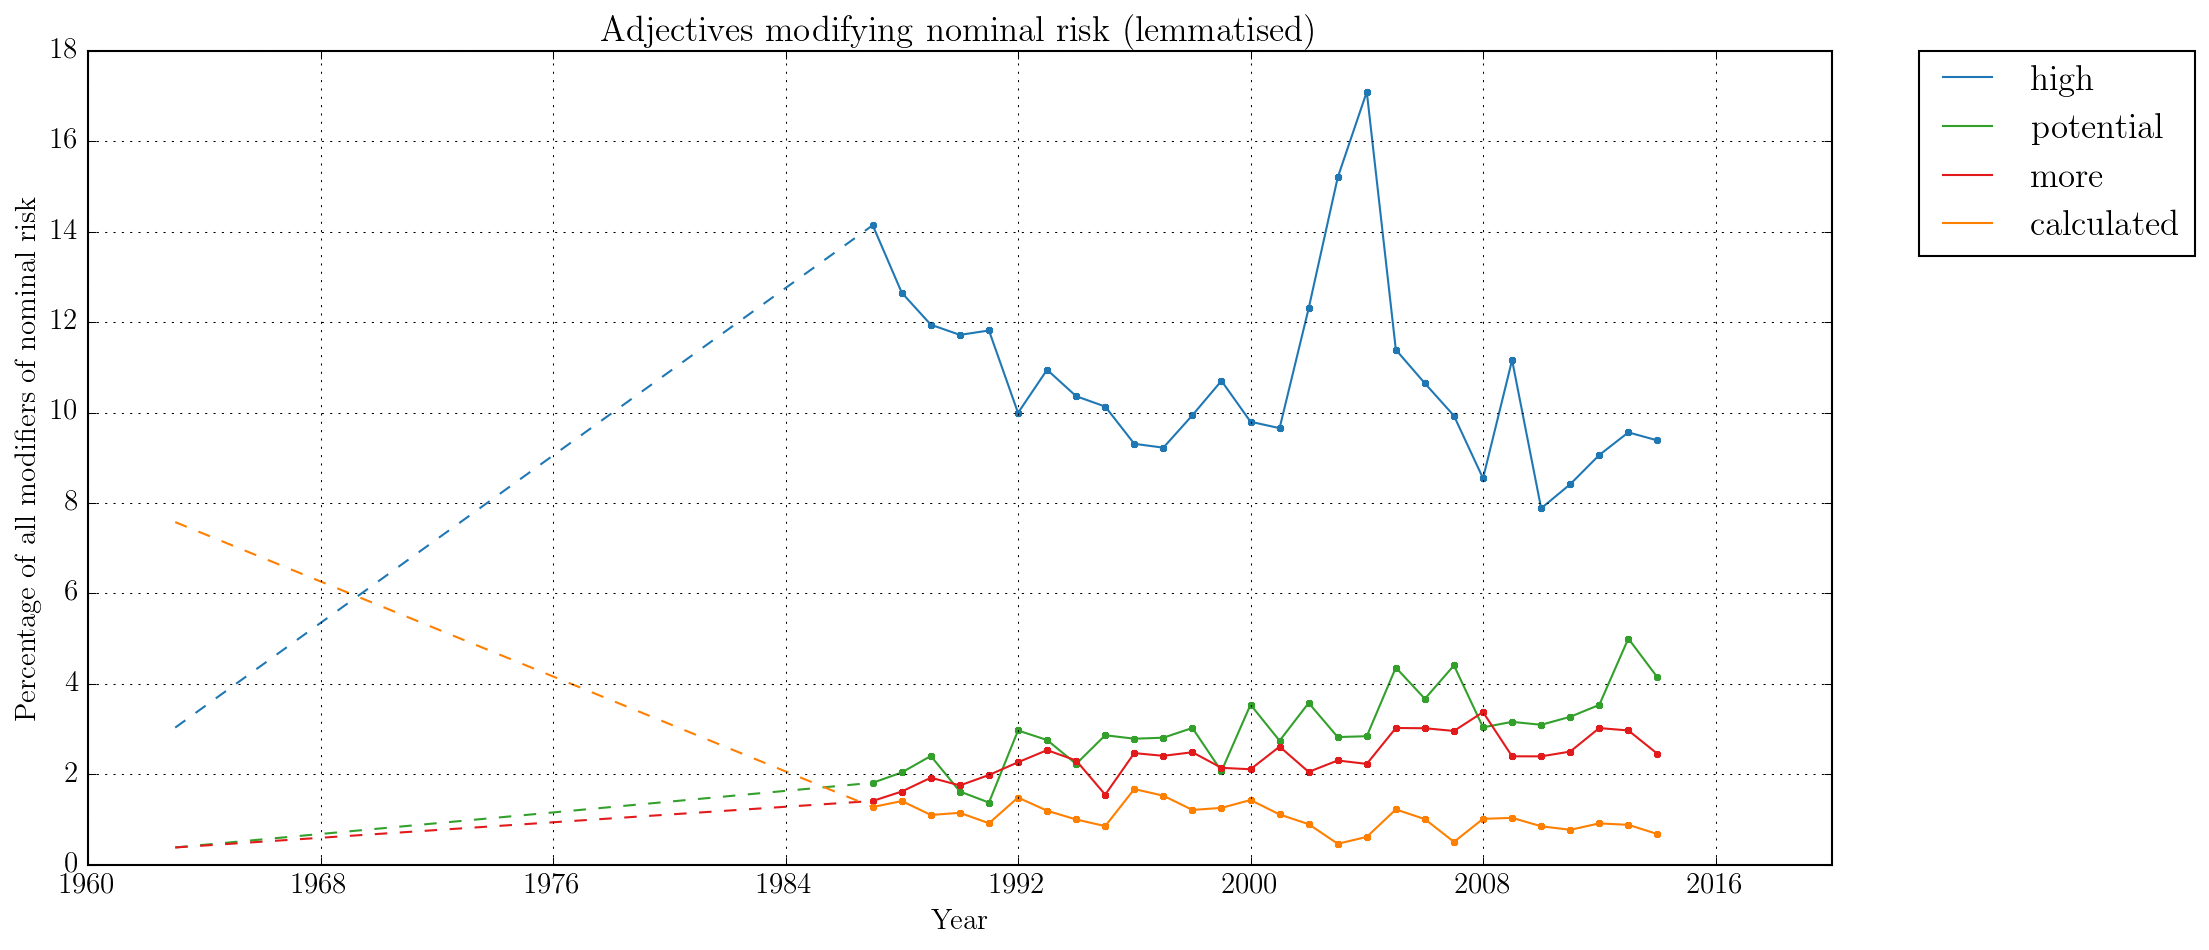
\includegraphics[width=0.75\textwidth]{../images/adjectives_modifying_nominal_risk_(lemmatised).png}
				\caption{Selected modifiers of participant risk as percentage of all risk modifiers}
				\label{fig:reladjrisk}
				\end{figure}

				%~\ \todo[inline,color=green!40]{\noindent Significance of this?}

		\section{What kinds of risk processes are there, and what are their relative frequencies?}
		\FloatBarrier

		Our second area of interest within the transitivity system is risk as a process. Within the corpus, we located five distinct risk processes. First, risk alone may be a process (\emph{I won't risk it}). Second and third are \emph{running risk} and \emph{taking risk}---\emph{process--range} configurations, where the verbal component is largely shorn of meaning, and with meaning conveyed primarily in the nominal in object position \cite{halliday_introduction_2004}. Fourth is \emph{putting somebody/something at risk}, which involves an obligatory nominal object argument and a prepositional-phrase complement. Finally, we have

        Other phrases sit on the cusp as recognisable risk processes: \emph{to carry risk}, for example, is frequent in the data, but we have not included it because we feel that the semantic burden of this process still lies in \emph{carry} (unlike \emph{pose} in \emph{to pose risk}).

			\begin{figure}[htb!]
			\centering
			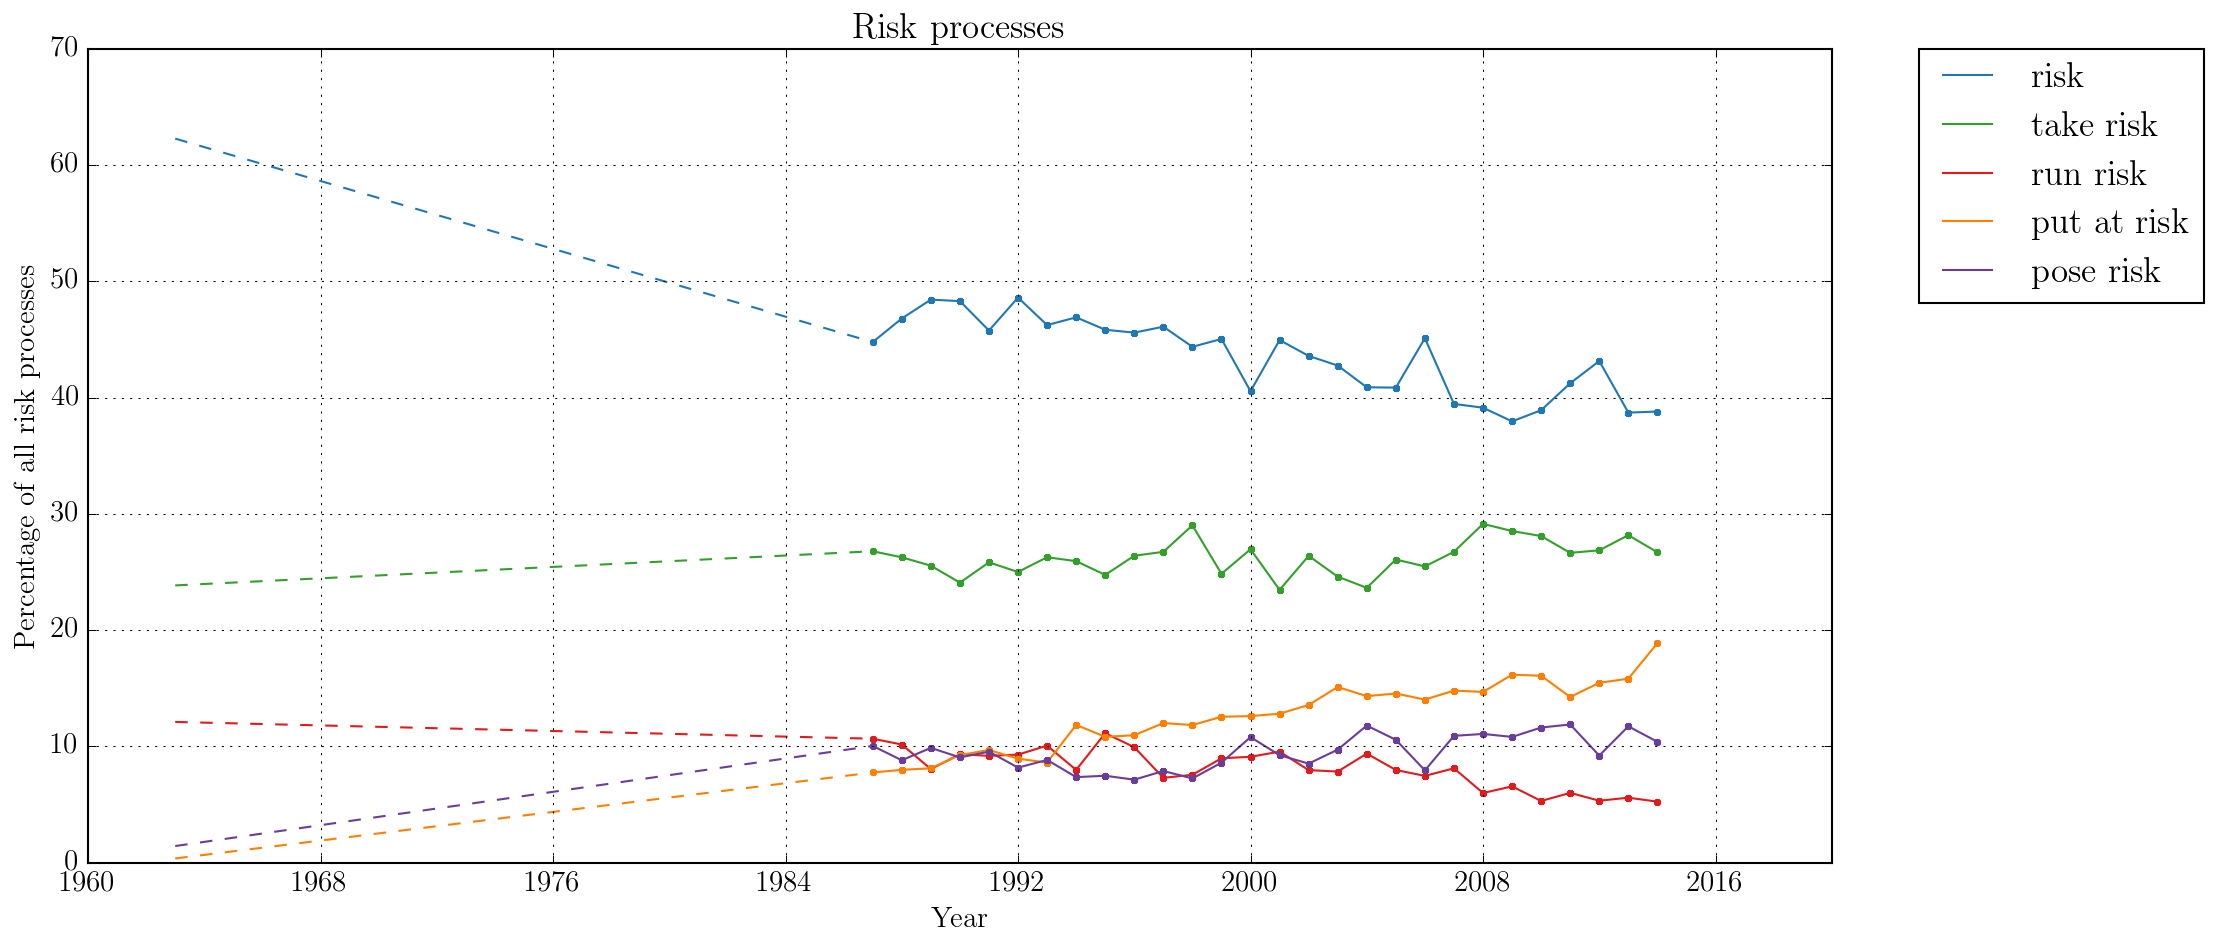
\includegraphics[width=0.75\textwidth]{../images/risk_processes.png}
			\caption{Risk processes as percentage of all parsed processes}
			\label{fig:riskprocesses}
			\end{figure}
			%
			Our first interest is the overall frequency of these five risk processes. 
            %From Figure \ref{fig:riskprocesses}, we concluded that risk processes generally are on an static\slash slightly outbound trajectory, with a notable decrease in frequency between the 1963--1987 samples.
            Figure \ref{fig:verbalrisks} charts the trajectory of the five identified risk processes. Most interesting here are that the `standard' (predicatorial) risk process is steadily decreasing, in favour of the other processes, each of which seems to provide additional connodations of the agency of the risker as well as his\slash her\slash its understanding of the level of risk. 

            The second notable finding here is that \emph{putting at risk} has overtaken \emph{running risk} in frequency.

             Concordancing revealed that in 2014, \emph{putting at risk} is used in cases where the potential harm is either implicit or explicit:

            \begin{enumerate}  [before=\itshape,font=\normalfont] \setlength\itemsep{0em} \small
                \item Ultimately, there is a price to pay: If you attack our soldiers, you're putting yourself at risk.
                \item But addicted health care workers need not be physicians to put patients at risk.
                \item While obviously no airline or company deliberately puts people at risk, `sometimes new risks are identified and steps have to be taken,' Mr. Koch said.
            \end{enumerate}

            \begin{enumerate}  [before=\itshape,font=\normalfont] \setlength\itemsep{0em} \small
                \item The auction houses deny that they are trimming profits with givebacks or putting themselves at financial risk.
                \item Rather, such tax status is generally put at risk when groups stray from their mission.
                \item They had handled her body, putting them at serious risk of infection.
            \end{enumerate}

            That said, we also noted that there seems to be some evidence for lessening agency in recent \emph{risk running} processes. Compare 1963 and 2014 results:

            \begin{enumerate} [before=\itshape,font=\normalfont]  \setlength\itemsep{0em} \small
            \item However, if adults decide to run a risk, this is up to them, and anyway, Switzerland adequately handles American affairs in Havana.
            \item In Washington at the weekend it was pretty welt agreed that the MIG incident was not deliberate provocation; the feeling was that, even with the Russian presence, Castro would not wilfully run the risk of American retaliation.
            \item  If he sticks to the more-or-less official Republican position against off-track betting, he runs the risk of losing thousands of New York City votes, which he needs.
            \end{enumerate}

            \begin{enumerate} [before=\itshape,font=\normalfont]   \setlength\itemsep{0em} \small
            \item Fans see this revolving door of injuries with so much regularity that they run the risk of becoming desensitized 
            \item `One runs the risk of falling for a voice.'
            \item `I would run the risk of having two boys,' she said.
            \item On the other hand, if Argentina does default, it runs the risk of more lawsuits, said Siobhan Morden, head of Latin America strategy at Jefferies.
            \item And, like an overdressed beachgoer, a classic cocktail served straight up runs a high risk of wilting in the sunshine.
            \end{enumerate}
            %
            Overall, the shift in both the semantics of risk running and the increasing preference for \emph{putting at risk} can be seen as evidence for decreasing agency in risk, as well as an increasing implicitness of the potential harm. This finding is especially significant, given that the existing descriptions of risk \cite{fillmore_toward_1992}, as well as the current FrameNet database, include accounts of \emph{running risk} as a frame, but not \emph{putting at risk}.
		
		\section{When risk is a process, what participants are involved?}
		\FloatBarrier
		
		Clauses containing risk processes are a rich site for analysis, as the semantic roles of participants are determined by their placement with respect to the process. Experiential subjects of risk processes can be mapped to \emph{riskers}. Experiential objects are either \emph{risked things} or \emph{potential harm} (\emph{they risked their lives/death}). Table \ref{tab:riskersx} lists the most common subject and object participants of risk processes. Also of interest are clauses embedded within risk processes (e.g. \emph{she risks hurting herself/losing her life}). Table \ref{alienating} lists the (lemmatised) top twenty subordinated processes in the corpus.

			\begin{table}[htb!]
			\centering
			\addvbuffer[12pt 8pt]{\begin{minipage}{.35\textwidth}
			\centering
			\small
			\begin{tabularx}{1.0\textwidth}{|>{\raggedright}l|X|}
			\hline
			\textbf{Risker}           & \textbf{Risked thing\slash potential harm} \\ \hline
			person & life \\ \hline
			company & injury \\ \hline
			state & loss \\ \hline
			woman & everything \\ \hline
			man & death \\ \hline
			investor & money \\ \hline
			bush & wound \\ \hline
			player & war \\ \hline
			government & career \\ \hline
			worker & arrest \\ \hline
			republican & health \\ \hline
			clinton & damage \\ \hline
			bank & reputation \\ \hline
			democrat & fine \\ \hline
			anyone & capital \\ \hline
			obama & future \\ \hline
			child & confrontation \\ \hline
			move & job \\ \hline
			firm & backlash \\ \hline
			administration & failure \\ \hline
			\end{tabularx}
			\caption{Riskers and risked things and\slash or potential harms}
			\label{tab:riskersx}

			\end{minipage}} \hspace{1cm} % This must go next to `\end{minipage}`
			\addvbuffer[12pt 8pt]{\begin{minipage}{.35\textwidth}

			\centering
			\small
			\begin{tabularx}{0.9\textwidth}{|l|X|}
			\hline
			\textbf{Embedded process}      & \textbf{Total ~~~~~~~~~~~~~~~~~~~~~~~~~~~~~~~~~~~~~~~~~~} \\ \hline
			lose      & 1260  \\ \hline
			be        & 1095  \\ \hline
			alienate  & 379   \\ \hline
			have      & 347   \\ \hline
			become    & 285   \\ \hline
			get       & 184   \\ \hline
			make      & 166   \\ \hline
			turn      & 119   \\ \hline
			go        & 113   \\ \hline
			offend    & 110   \\ \hline
			take      & 86    \\ \hline
			look      & 85    \\ \hline
			undermine & 82    \\ \hline
			anger     & 79    \\ \hline
			fall      & 78    \\ \hline
			create    & 76    \\ \hline
			put       & 74    \\ \hline
			miss      & 73    \\ \hline
			give      & 73    \\ \hline
			damage    & 62    \\ \hline
			\end{tabularx}
			\caption{Most common embedded processes in risk processes}
			\label{alienating}
	
			\end{minipage}}
			\end{table}

			Riskers are most typically powerful institutions or individuals. Risked things and potential harms are generally serious and grave. A mismatch occurs here: \emph{Bush} and \emph{Obama} do not likely risk \emph{wounds}, \emph{arrest} or \emph{death}. In terms of subordinated processes, notable is the appearance of processes that are fairly uncommon: \emph{alienating}, \emph{offending}, \emph{undermining} and \emph{angering} and are three key examples, ranking amongst expected processes like \emph{being}, \emph{having}, \emph{getting}, \emph{making} and \emph{going}. Without considering longitudinal change, we can see from this that the embedded processes are often related to more powerful social actors: states, political parties and politicians risk alienating electorates; diplomats risk offending one another. Even embedded processes lacking explicit connotations of power are typically deployed in the contexts of government, industry or society. Below are concordance results for \emph{risk alienating} in 2013, which appears 14 times.


            \begin{figure}
            \footnotesize
            \begin{tabular}{rcl}
    stoked further concerns that unemployment risked &  becoming &  endemic and could eventually cause social upheaval  \\ 
     franchise, the stage scene could have risked &  becoming &  an embarrassment for the brand, but Mr. Timbers'   \\ 
   with locally, or else the Vatican offices risk &  becoming &  institutions of censorship   \\ 
           on which the experience depends -- or risk &  becoming &  irrelevant to future generations, Mr. Staggs said   \\ 
   restart growth, warning that the euro area risked &  becoming &  mired in the same kind of economic stagnation that   \\ 
            If left unaddressed, such practices risk &  becoming &  more and more entrenched, Ann Harrison of   \\ 
    without serious savings in this area, we risk &  becoming &  an unbalanced force, one that is well compensated   \\ 
                                    Switzerland risks &  becoming &  one of the most restrictive places for management   \\ 
              What was the exception before now risks &  becoming &  the standard practice   \\ 
       the pope's new remarks that the church risked &  becoming &  a `small chapel' overly fixated on sexual   \\ 
            hailed the step as significant, it risks &  becoming &  the latest of many tentative moves toward talks   \\ 
      Rather than race the clock to Bed-Stuy and risk &  becoming &  an early bike-share casualty, I stopped at a   \\ 
   increasingly turning to what, strangely, risked &  becoming &  the most marginalized group of all: the bosses   \\ 
    and currency crisis in the European Union risks &  becoming &  a crisis of liberal democracy itself \\ 
            \end{tabular}
            \caption{\emph{To risk becoming} in 2013 subcorpus}
            \end{figure}
			

			%DEPENDING ON HOW MUCH TIME THERE IS, I COULD SEARCH FOR ALL OF THE RISKERS INDIVIDUALLY...

			%Though these objects may be grammatically ambiguous, the function of the object can be disambiguated by inserting \emph{losing}.

			%\begin{enumerate}	\setlength\itemsep{0em}
				%\item He risked his life
				%\item He risked losing his life
				%\item He risked death
				%\item * He risked losing death
			%\end{enumerate}

			%Note here an emerging methodological issue: the various  \emph{potential harms} can also be located by querying nominal risks (e.g. \emph{the risk of death}). Some methodological adaptability is thus required.

		\section{When risk is a modifier, what are the most common forms?} \label{sect:riskmod}
		\FloatBarrier

            \begin{table}
            \small
            \centering
            \begin{tabular}{|l|l|}
            \hline
            \textbf{Modifier type}       & \textbf{Example}          \\ \hline
            Adjectival pre-head & \emph{a risky move}     \\ \hline
            Post-head           & \emph{A person at risk} \\ \hline
            pre-head nominal    & \emph{risk management}  \\ \hline
            Adverbial           & \emph{to riskily act}   \\ \hline
            Circumstance head   & \emph{to be at risk }   \\ \hline
            \end{tabular}
            \caption{Types of risk-as-modifier}
            \label{tab:modriskwords}
            \end{table}

            There are many different kinds of risk as modifier (see Table \ref{tab:modriskwords} for a non-exhaustive list of examples). Our first interest was in gauging the prevalence of the different forms. From this query, we noted that pre-head nominal modifiers are increasing in frequency. A good example is \emph{risk factor} (see Figure \ref{fig:riskfactor}).


          \noindent
          \begin{figure}[htb!]
          \centering
          \begin{minipage}{.567\textwidth}
            \centering
            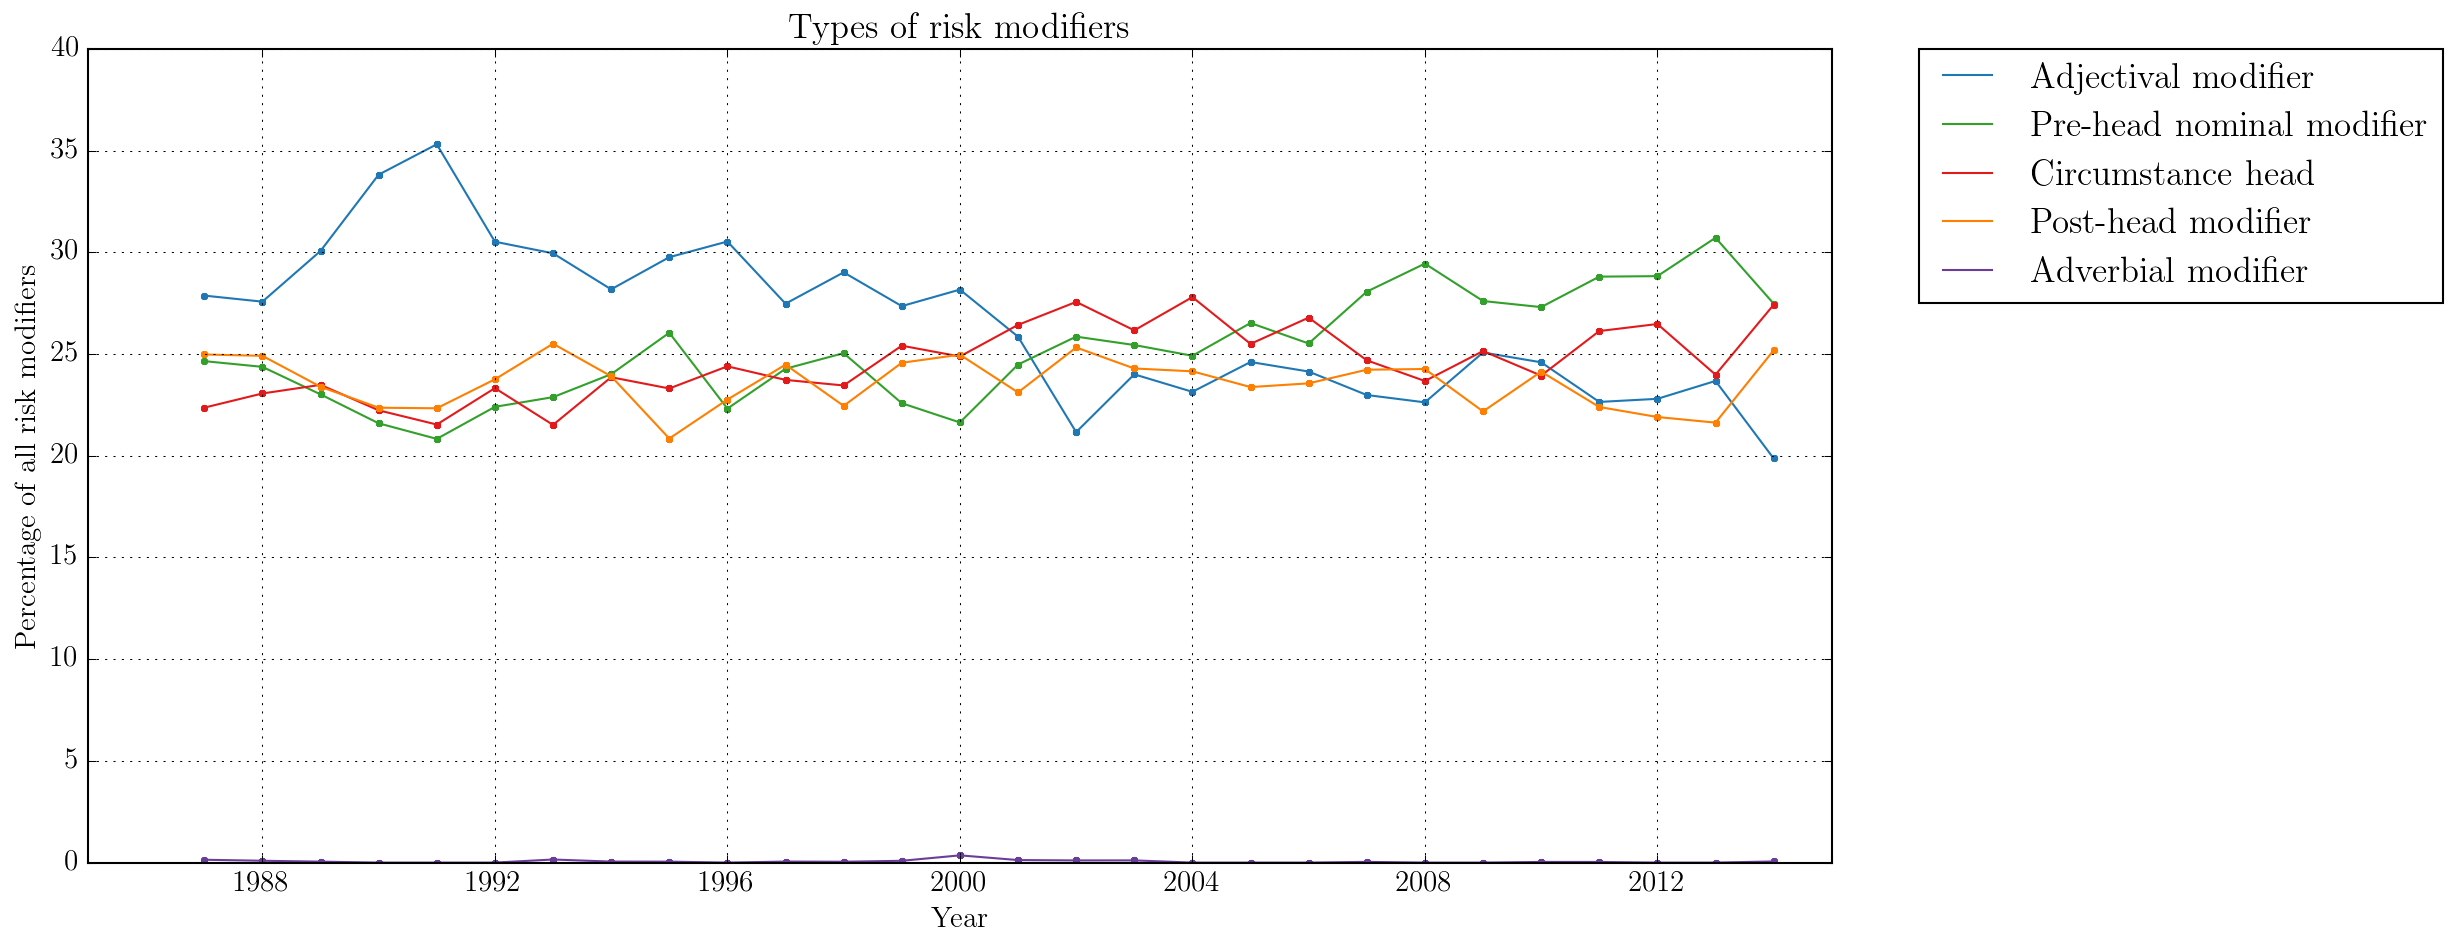
\includegraphics[width=0.98\textwidth]{../images/types-of-risk-modifiers.png}
         \captionof{figure}{Types of risk modifier}
         \label{fig:riskmod_types}
          \end{minipage}%
          \begin{minipage}{.433\textwidth}
            \centering
              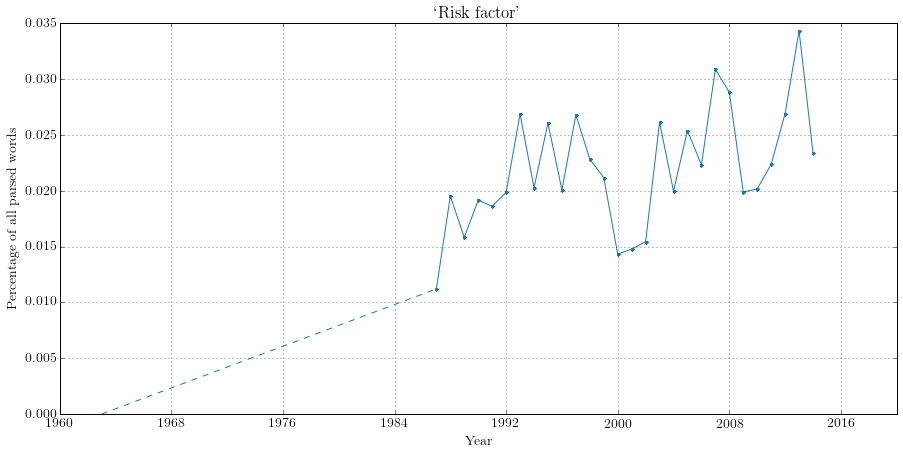
\includegraphics[width=0.98\textwidth]{../images/risk-factor.png}
              \captionof{figure}{Relative frequency of \emph{risk factor}}
                \label{fig:riskfactor}
           \end{minipage}
          \end{figure}


			Modifier risks are unique for their variety and diversity: through compounding, comprehensible new risk words and phrases can easily be created. The entire corpus contained 327 unique adjectival risk words, including \emph{non-risk}, \emph{de-risk}, \emph{once-risky}, \emph{take-no-risks}, \emph{risk-swapping}, \emph{risk-abhorrent}, \emph{price-for-risk}, \emph{post-risky}, \emph{pooled-risk}, \emph{personal-risk}, \emph{optimum-risk}, \emph{one-risk-factor}, \emph{one-pitch-can-end-his-career-risk} and \emph{low-risk-to-society}. That said, most of these occur no more than a handful of times. By far the most common were \emph{risky\slash riskier\slash riskiest} (15588 occurrences), \emph{high-risk} (5533), \emph{low-risk} (1086), \emph{at-risk} (902), \emph{risk-free} (883) and \emph{risk-taking} (789). Of these, four exhibited trajectory shifts (see Figure \ref{fig:adjtraj}). The basic adjectival forms (\emph{risky}, \emph{riskier}, \emph{riskiest}) are dominant in the 1963 sample, then decrease, and re-emerge in 2000. \emph{High-risk} though very rare (two instances) in 1963, has become more common, and stabilised in trajectory. \emph{Low-risk} and \emph{at-risk} are on a consistent inbound trajectory.

            \noindent
          \begin{figure}[htb!]
          \centering
          \begin{minipage}{.48\textwidth}
            \centering
            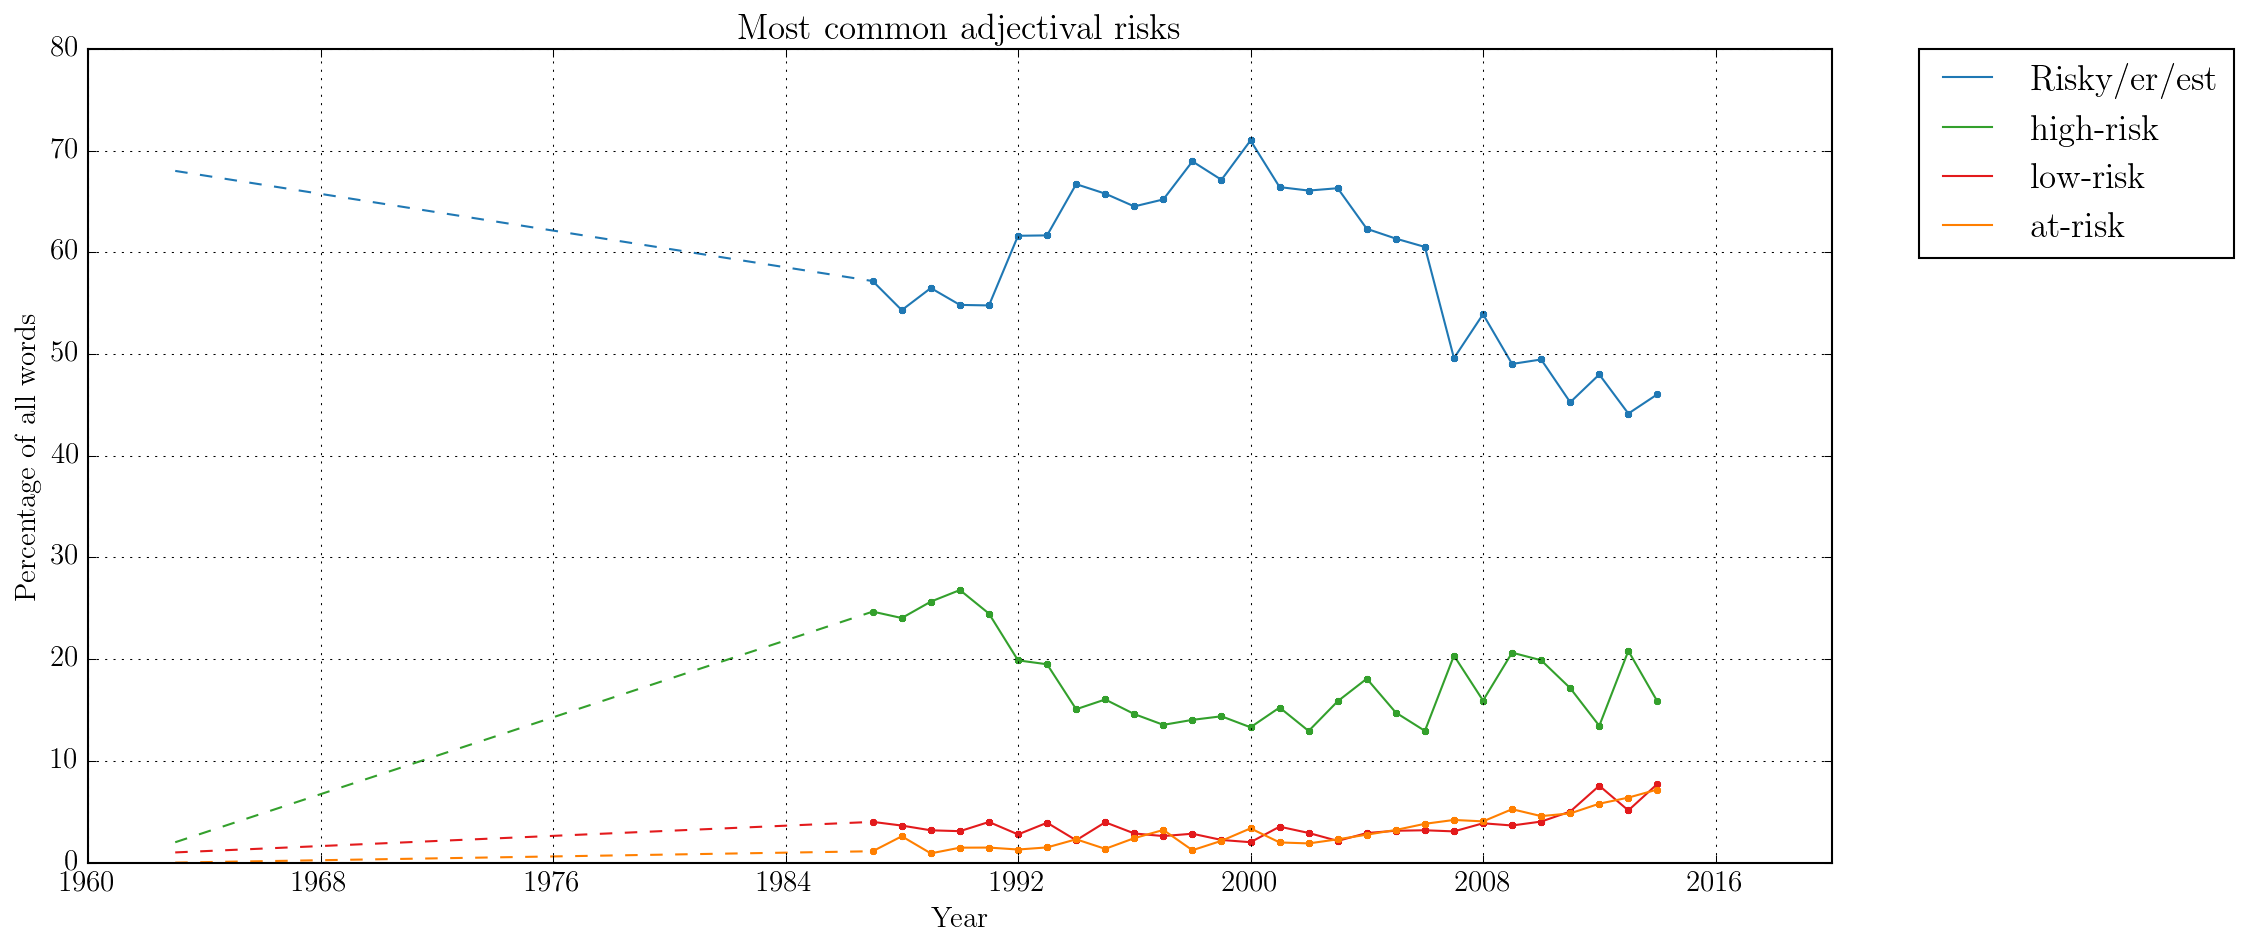
\includegraphics[width=0.98\textwidth]{../images/most_common_adjectival_risks.png}
          \end{minipage}%
          \begin{minipage}{.48\textwidth}
            \centering
            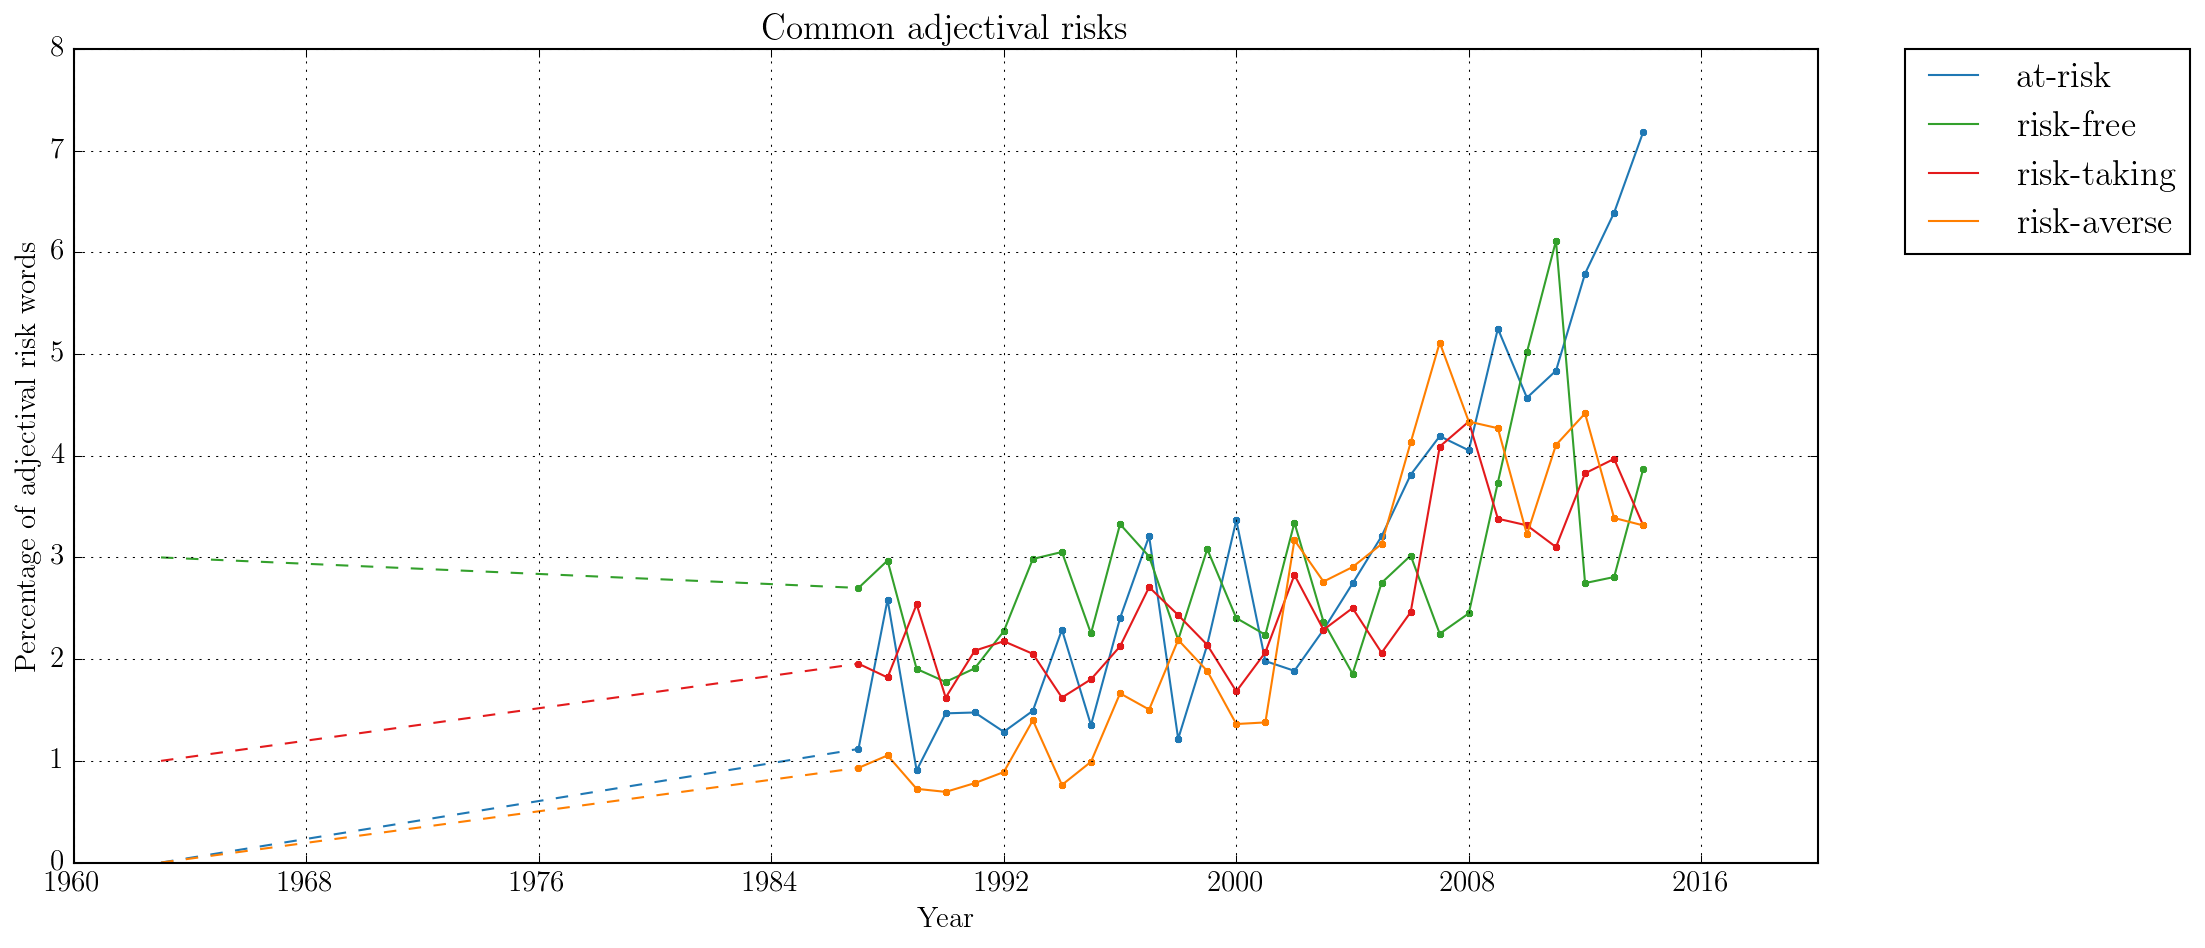
\includegraphics[width=0.98\textwidth]{../images/common_adjectival_risks.png}
           \end{minipage}
           \caption{Common adjectival risk words as percentage of all adjectival risks}
                \label{fig:adjtraj}
          \end{figure}


			The prevalence of high-risk in the 1980s is largely due to the AIDS epidemic: concordancing reveals that certain populations (gays, African Americans, Haitians) are at high-risk of being inflected by HIV. \emph{At-risk} is rare in earlier editions, but increases in prevalence steadily.

			This shift in risk is modifier is an important one. Low, moderate and high risk comprises a gradient, or scale, while at-risk is a binary. As with the shift toward \emph{potential risk}, this indicates both an increasing pervasiveness and a decreasing calcuability of risk. %remember that low-risk is actually increasing.
			
			%Of the graduated risks, low-risk is the only one on an inbound trajectory. What's the significance of this?



				%For people at moderate risk who also have two of the other risk factors , the treatment should be the same as for those in the high-risk group .
				%But ecologists , doctors and other specialists here warn that the entire population , not just high-risk groups , is vulnerable .
				%In the weeks since the law took effect , couples seeking marriage licenses have besieged hospitals , clinics and other doctors , anxious to get the test and the required counseling in time for wedding dates and quickly outnumbering those in high-risk groups most in need of attention .
				%Health experts say scarce funds for AIDS prevention would be better spent on high-risk groups .
				%Very few Americans know that Haitians have long since been removed from the list of high-risk groups because it was discovered that the H


			\section{When risk is a modifier, what is being modified?}
			\FloatBarrier

			Risk as a modifier can be placed either before or after the noun it modifies (\emph{an at-risk person\slash a person at risk}). These two constructions are collapsed in Tables \ref{tab:riskmodified} and \ref{tab:atrisk}, which respectively list the participants most frequently modified by any risk modifier, and the participants most frequently modified by \emph{at-risk\slash at risk}. Note that while risk-modified participants generally are financial and economic in nature (\emph{investment, business, loan, asset}), the at-risk subset is comprised of vulnerable populations of people (\emph{women}, \emph{children}, \emph{students}).

			\begin{table}[htb!]
			\centering
			\addvbuffer[12pt 8pt]{\begin{minipage}{.37\textwidth}
			\centering
			\small
			\begin{tabularx}{1.0\textwidth}{|X|l|}
			\hline
			\textbf{Risk-modified \mbox{participant}}        & \textbf{Total} \\ \hline
			investment  & 696   \\ \hline
			business    & 515   \\ \hline
			behavior    & 508   \\ \hline
			group       & 466   \\ \hline
			loan        & 421   \\ \hline
			asset       & 388   \\ \hline
			strategy    & 377   \\ \hline
			bond        & 346   \\ \hline
			area        & 307   \\ \hline
			venture     & 301   \\ \hline
			security    & 287   \\ \hline
			patient     & 265   \\ \hline
			pool        & 239   \\ \hline
			bet         & 214   \\ \hline
			move        & 204   \\ \hline
			activity    & 201   \\ \hline
			proposition & 199   \\ \hline
			child       & 170   \\ \hline
			woman       & 161   \\ \hline
			student     & 158   \\ \hline
			\end{tabularx}
			\caption{Most common risk-modified participants in the corpus}
			\label{tab:riskmodified}
			\end{minipage}} \hspace{1cm}
			\addvbuffer[12pt 8pt]{\begin{minipage}{.37\textwidth}
			\small
			\begin{tabularx}{1.0\textwidth}{|X|l|}
			\hline
			\textbf{At-risk \mbox{participant}}       & \textbf{Total} \\ \hline
			person     & 439   \\ \hline
			child      & 368   \\ \hline
			woman      & 209   \\ \hline
			student    & 179   \\ \hline
			nation     & 135   \\ \hline
			patient    & 110   \\ \hline
			youngster  & 93    \\ \hline
			group      & 91    \\ \hline
			population & 64    \\ \hline
			family     & 58    \\ \hline
			kid        & 50    \\ \hline
			youth      & 48    \\ \hline
			money      & 48    \\ \hline
			worker     & 45    \\ \hline
			life       & 41    \\ \hline
			job        & 41    \\ \hline
			man        & 40    \\ \hline
			area       & 35    \\ \hline
			teenager   & 32    \\ \hline
			other & 32 \\ \hline
			\end{tabularx}
			\caption{Most common at-risk participants in the corpus}
			\label{tab:atrisk}
			\end{minipage}}% This must go next to `\end{minipage}`
			\end{table}

        In need of further research is whether or not the list of entities that can sensibly be modified by \emph{at-risk} is beginning to grow: since the U.S. subprime mortgage crisis (beginning in 2007), references to \emph{at-risk homeowners} appear to be on the rise. Results from 2011, for example, show that \emph{nations} and even \emph{economic sectors} are being modified with \emph{at-risk}:

        \begin{enumerate}  [before=\itshape,font=\normalfont] \setlength\itemsep{0em} \small
            \item Mr. Obama asked for \$400 million for the World Bank's clean technology fund, \$95 million for the bank's program to prevent deforestation and \$90 million for its program to help at-risk nations cope with the effects of a warming planet by, for instance, developing drought-resistant crops.
            \item The most at-risk sectors included auto components and automobile companies, which generate nearly 30 percent of their sales in Europe, as well as food and tobacco firms.
        \end{enumerate}

        Note that it is difficult to reconcile the semantic meaning of \emph{at-risk} constructions with the semantic frame of risk provided by \citeA{fillmore_toward_1992}. Though elements of both the \textsc{victim} and \emph{valued object} appear to be at work, neither provides an adequate label for \emph{at-risk people, children, homeowners or nations}. Rather than being an oversight during the articulation of the risk frame (recall Figure~\ref{fig:fil_atk}), in light of the increased use of these kinds of constructions since the mid 1990s, we hypothesise that \emph{at-risk} constructions (as well as \emph{to put at risk}) are demonstrative of a broader shift in risk discourse toward general clusters of negative outcomes, rather than specific and measurable potential harms. Connection between this shift and sociological theory is made in the following chapter.
        
	\section{How arguable is risk?} \label{sect:arguability}
	\FloatBarrier

		As noted earlier, our central concern with the Mood system is the degree of arguability associated with the concept of risk. Risk in Subject, Finite and Predicator positions is the most arguable. Risk words within Complements and Adjuncts are less arguable.

		%A dependency grammar attempts to locate a lexical root for each clause, and attach dependents to it recursively until no lexical items are unattached. Each word is ordered by its dependency to the root of a clause. The nature of the dependency relationship can also be provided. Such grammars are particularly useful for free word order language, but have been applied to English successfully as well.

		Based on the kinds of parsing provided by Stanford CoreNLP, it was possible to measure arguability in two ways. First, we can map dependency relationships to the systemic-functional notion of arguability. A dependency grammar locates the predicator of a clause and assigns it a position of zero. A `1' is then assigned to its most immediate dependent (other components in the verbal group, if present, or the head of the Subject, if not). This process continues until no lexical items are unattached, or `ungoverned'. In effect, the higher the number attached to a word, the further it is semantically from being an important component in the meaning, and thus, in systemic functional terms, the less arguable the word.

			\begin{figure}[htb!]
			\centering
			\addvbuffer[12pt 8pt]{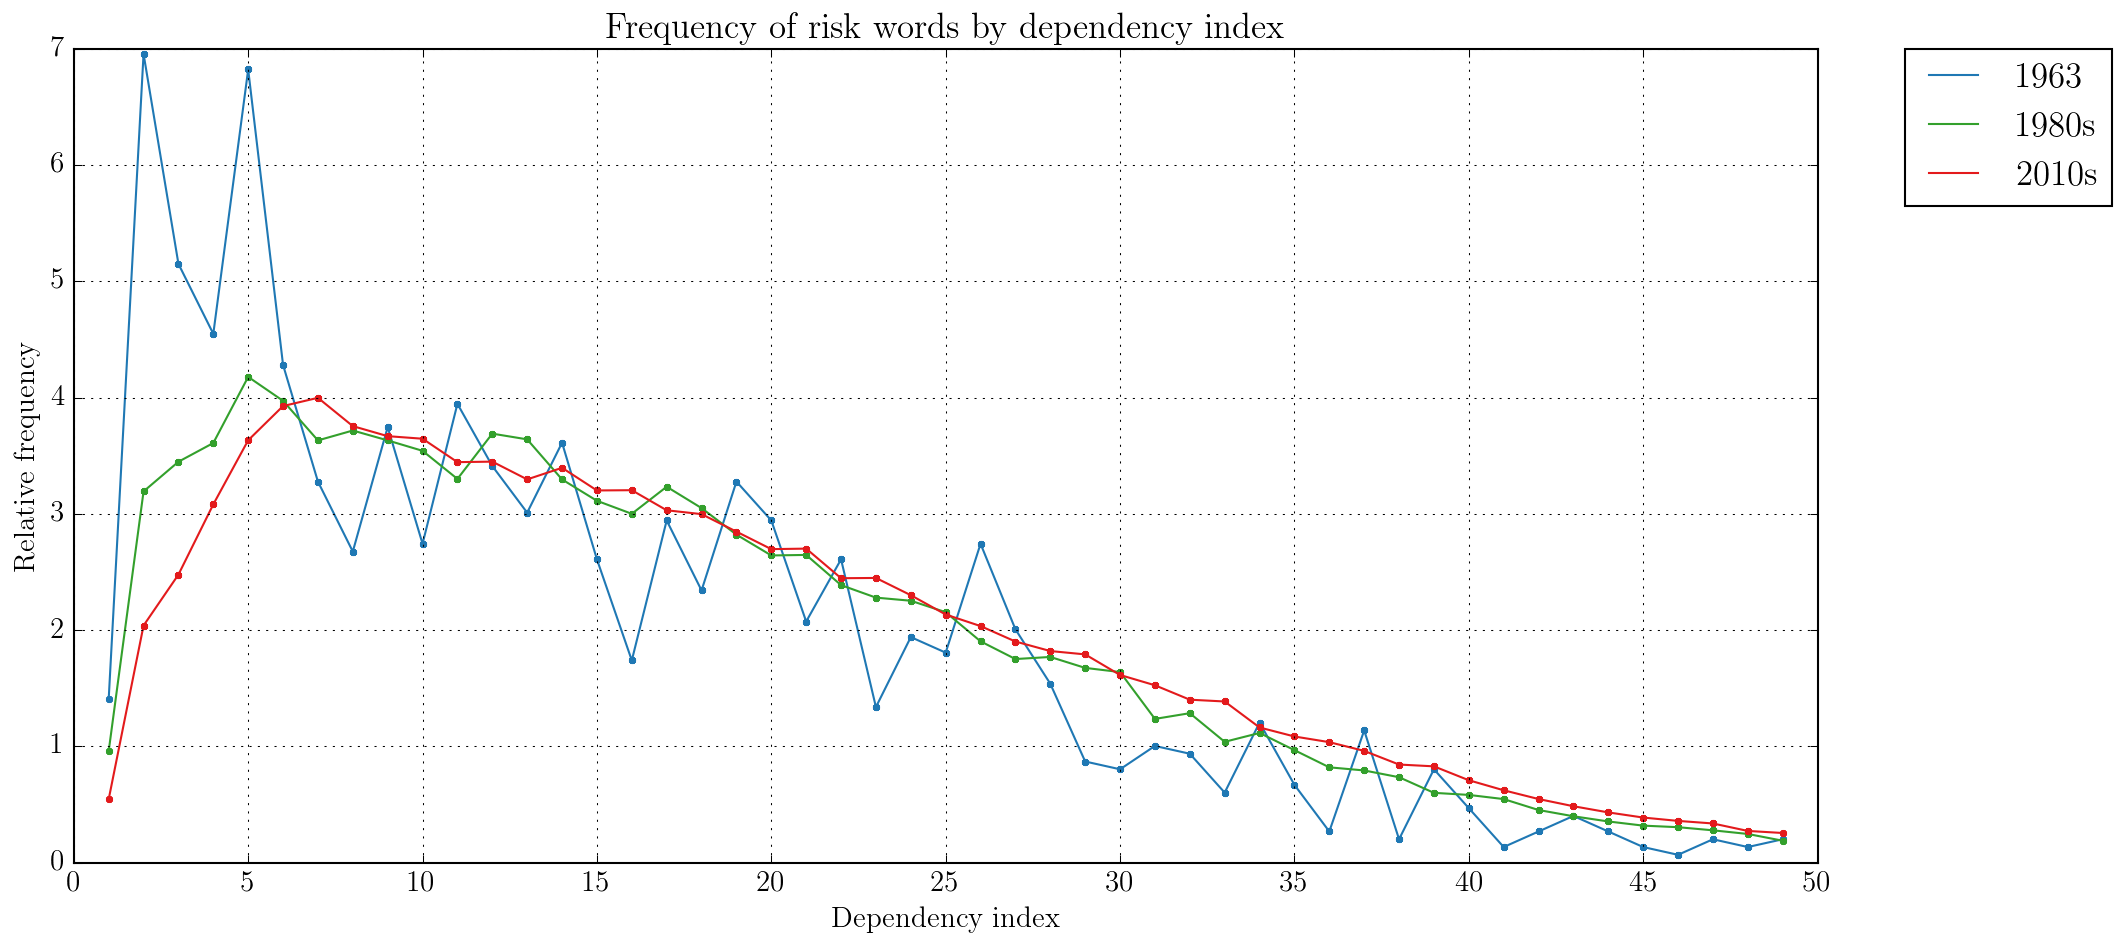
\includegraphics[width=0.75\textwidth]{../images/frequency-of-risk-words-by-dependency-index.png}}
			\caption{Risk words by dependency position in clause}
			\label{fig:depnum}
			\end{figure}
			%
			Highlighting three sampling periods as in Figure \ref{fig:depnum} shows that in early samples, risk occupies core roles within the dependency hierarchy, and thus sits closer to the core part of the meaning being exchanged within the clause. In later samples, risk more commonly occurs later in the dependency structure, in less focial positions. As explained earlier, though this experimental method is not a perfectly reliable indicators of arguability, it does indicate an increasing preference to position risk as non-core, ancillary information, rather than as the main thing which is under discussion.

            %\endnote{Dependency place 2 and 3 removed from visualisation, as these roles are typically for finites and modal auxiliaries---positions that a risk word cannot grammatically fill.}

			The second thing we can use dependency output for is identifying the functional roles of risk words. This is more accurate than using the dependency ranking, but creates a long list of functional roles. Of key interest, however, are risk words at the head of each major component of the Mood system---Subject, Finite\slash Predicator, Complement and Adjunct (CoreNLP parses unfortunately do not distinguish between Finite and Predicator in a reliable way, so the categories are collapsed here). From Figure \ref{fig:interpersonalarg}, we can see that risk is shifting from Subject and Finite\slash Predicator to Complement and Adjunct roles. This is an important result: risk words in more arguable roles are steadily decreasing, while risk in less arguable roles are becoming more common. Like earlier findings, this suggests an increasing implicitness of risk in NYT discourse, with less talk actually \emph{about} risk, but more talk where the relationship between risk and the subjects of the talk is assumed to be more or less common knowledge.

                      \noindent
          \begin{figure}[htb!]
          \centering
          \begin{minipage}{.48\textwidth}
            \centering
            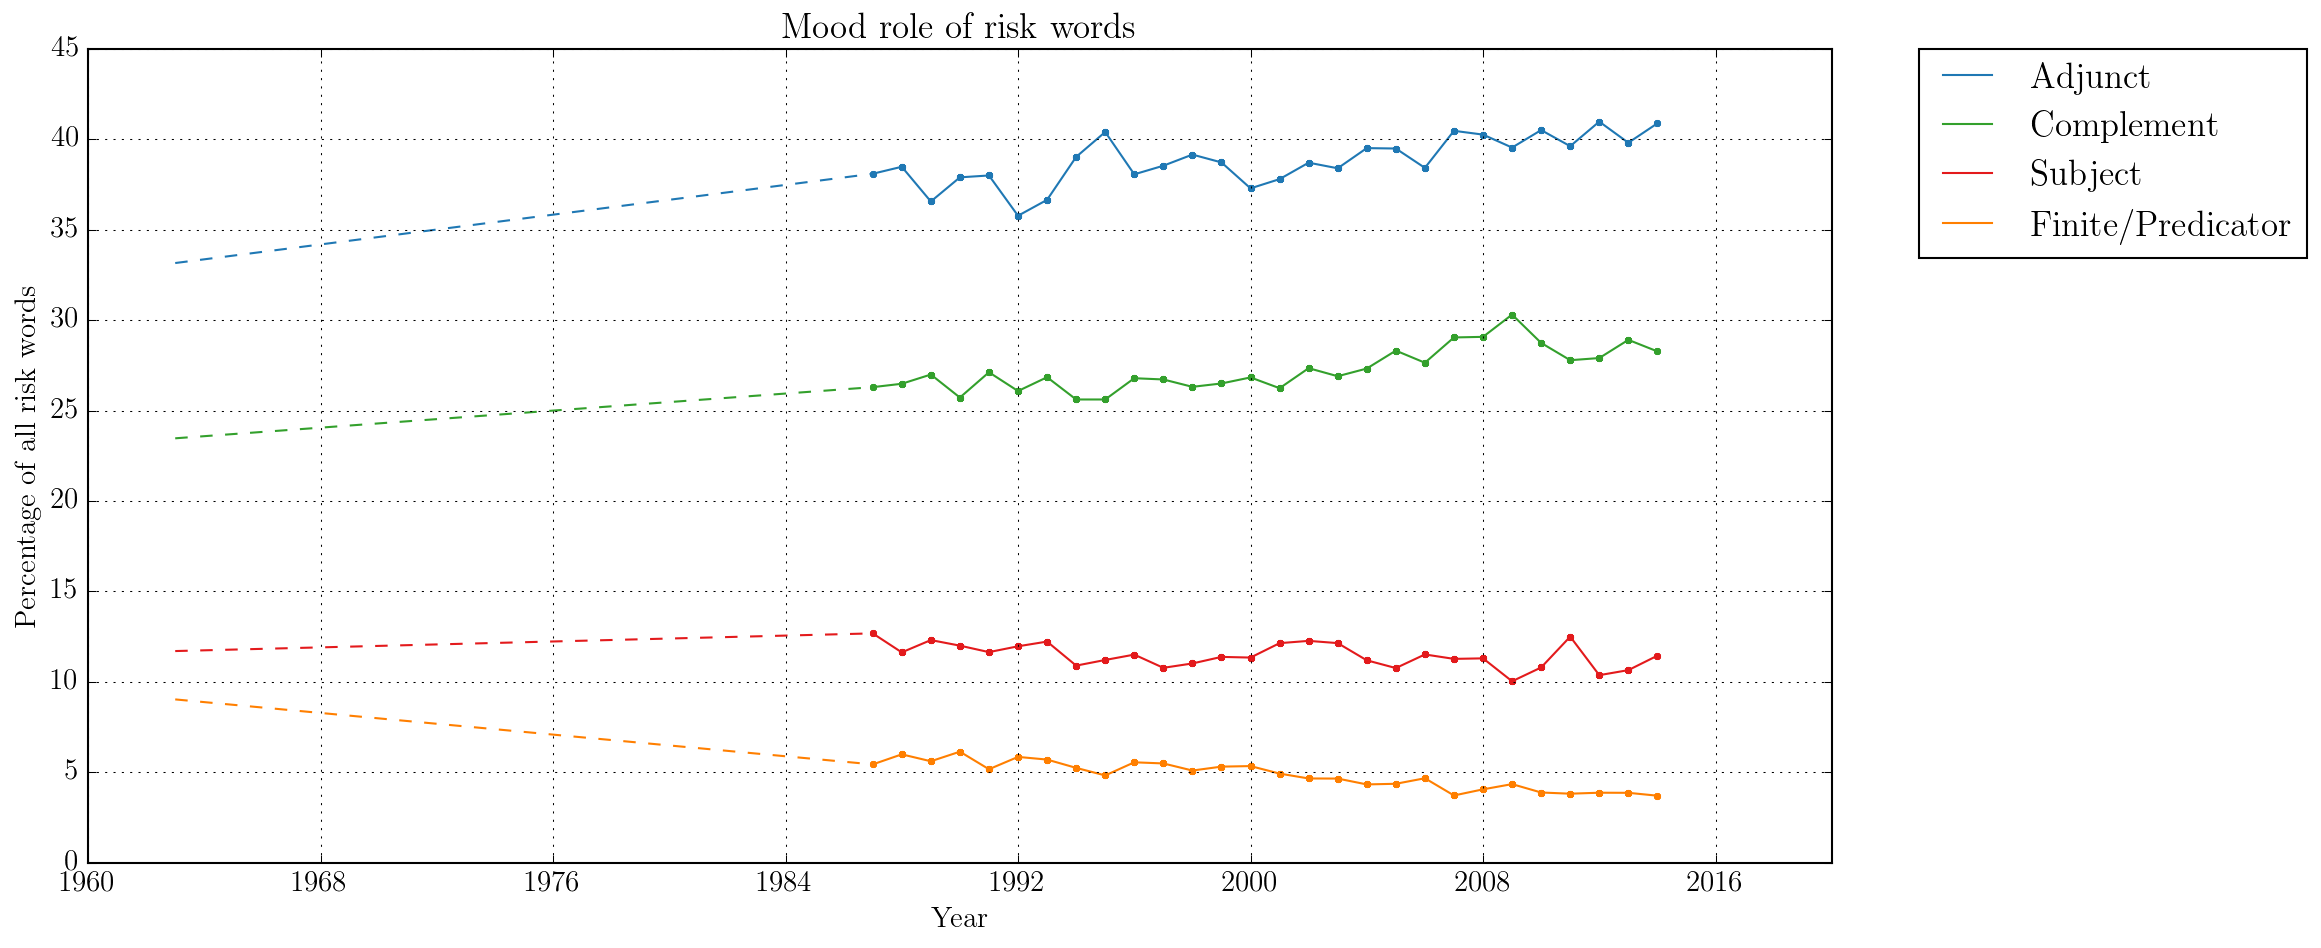
\includegraphics[width=0.98\textwidth]{../images/mood_role_of_risk_words.png}
          \end{minipage}%
          \begin{minipage}{.48\textwidth}
            \centering
            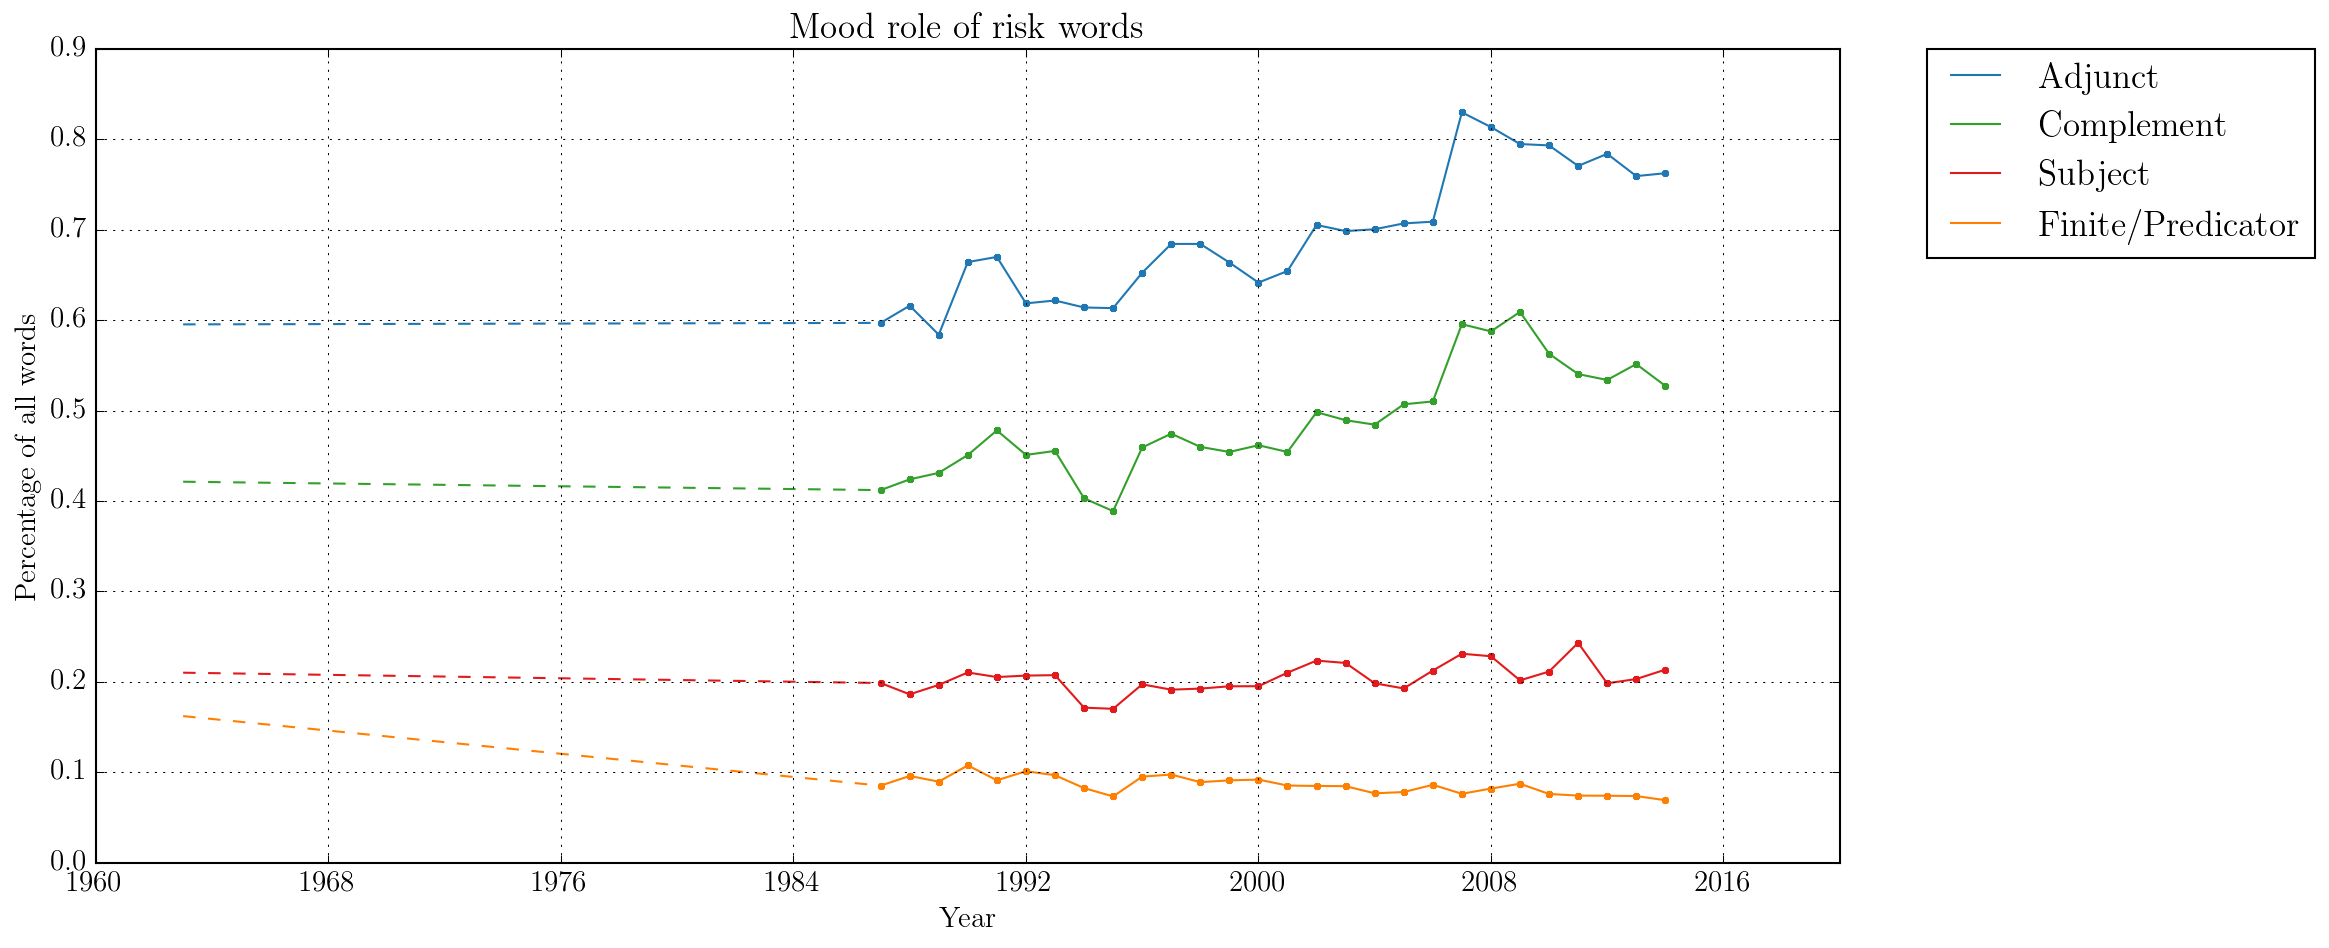
\includegraphics[width=0.98\textwidth]{../images/riskdep_allwords.png}
           \end{minipage}
            \caption{Frequency of risk words for each Mood component as percentage of all risk words\slash all parsed data}
            \label{fig:interpersonalarg}
          \end{figure}

            %By providing each role with a relative weight, we can plot arguability as a single decreasing trend line, showing the increased implicitness of risk within the language of the NYT.

			%Using the full list of risk dependencies, we can also locate more specific constructions undergoing trajectory shift. Figure \ref{fig:salienttrajectories} shows that risk is increasingly instantiated within prepositional phrases (which are by their nature dependent on Participants and Processes), and decreasingly as a predicator. From this view too, risk words are increasingly implicit within news language.

	\section{Risk words and proper nouns}

                We searched for proper noun groups in parse trees containing a risk word. This is a departure from many of our earlier queries, as here we are looking only at which entities co-occur with risk language, rather than determining how risk words and non-risk words relate to other another lexicogrammatically. The result of this query was 68891 different proper noun groups. We took the 200 most common results, and merged any that denoted the same entity: \emph{F.D.A.\slash Food and Drug Administration}, or \emph{Federal Reserve and Fed}. We then grouped results into thematic categories: \emph{People}, \emph{Nations}, \emph{Geopolitical entities}, \emph{Companies}, \emph{Organisations} and \emph{Medical themes}. The results were then plotted (See Figure \ref{fig:propernouns}). 

                  \begin{landscape}
                  \centering
                  \begin{figure}
                  \captionsetup[subfigure]{oneside,margin={-1.5cm,-.5cm}}
                  \centering % [t!] % "[t!]" placement specifier just for this example
                  \begin{subfigure}{.64\textwidth}
                  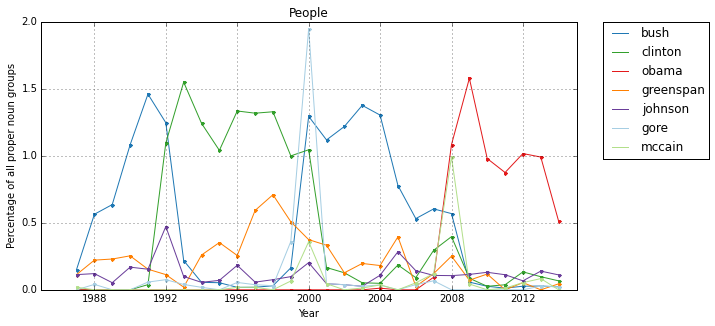
\includegraphics[width=\linewidth]{../images/people}
                  \caption{People} \label{fig:a}
                  \end{subfigure}
                  \begin{subfigure}{.64\textwidth}
                  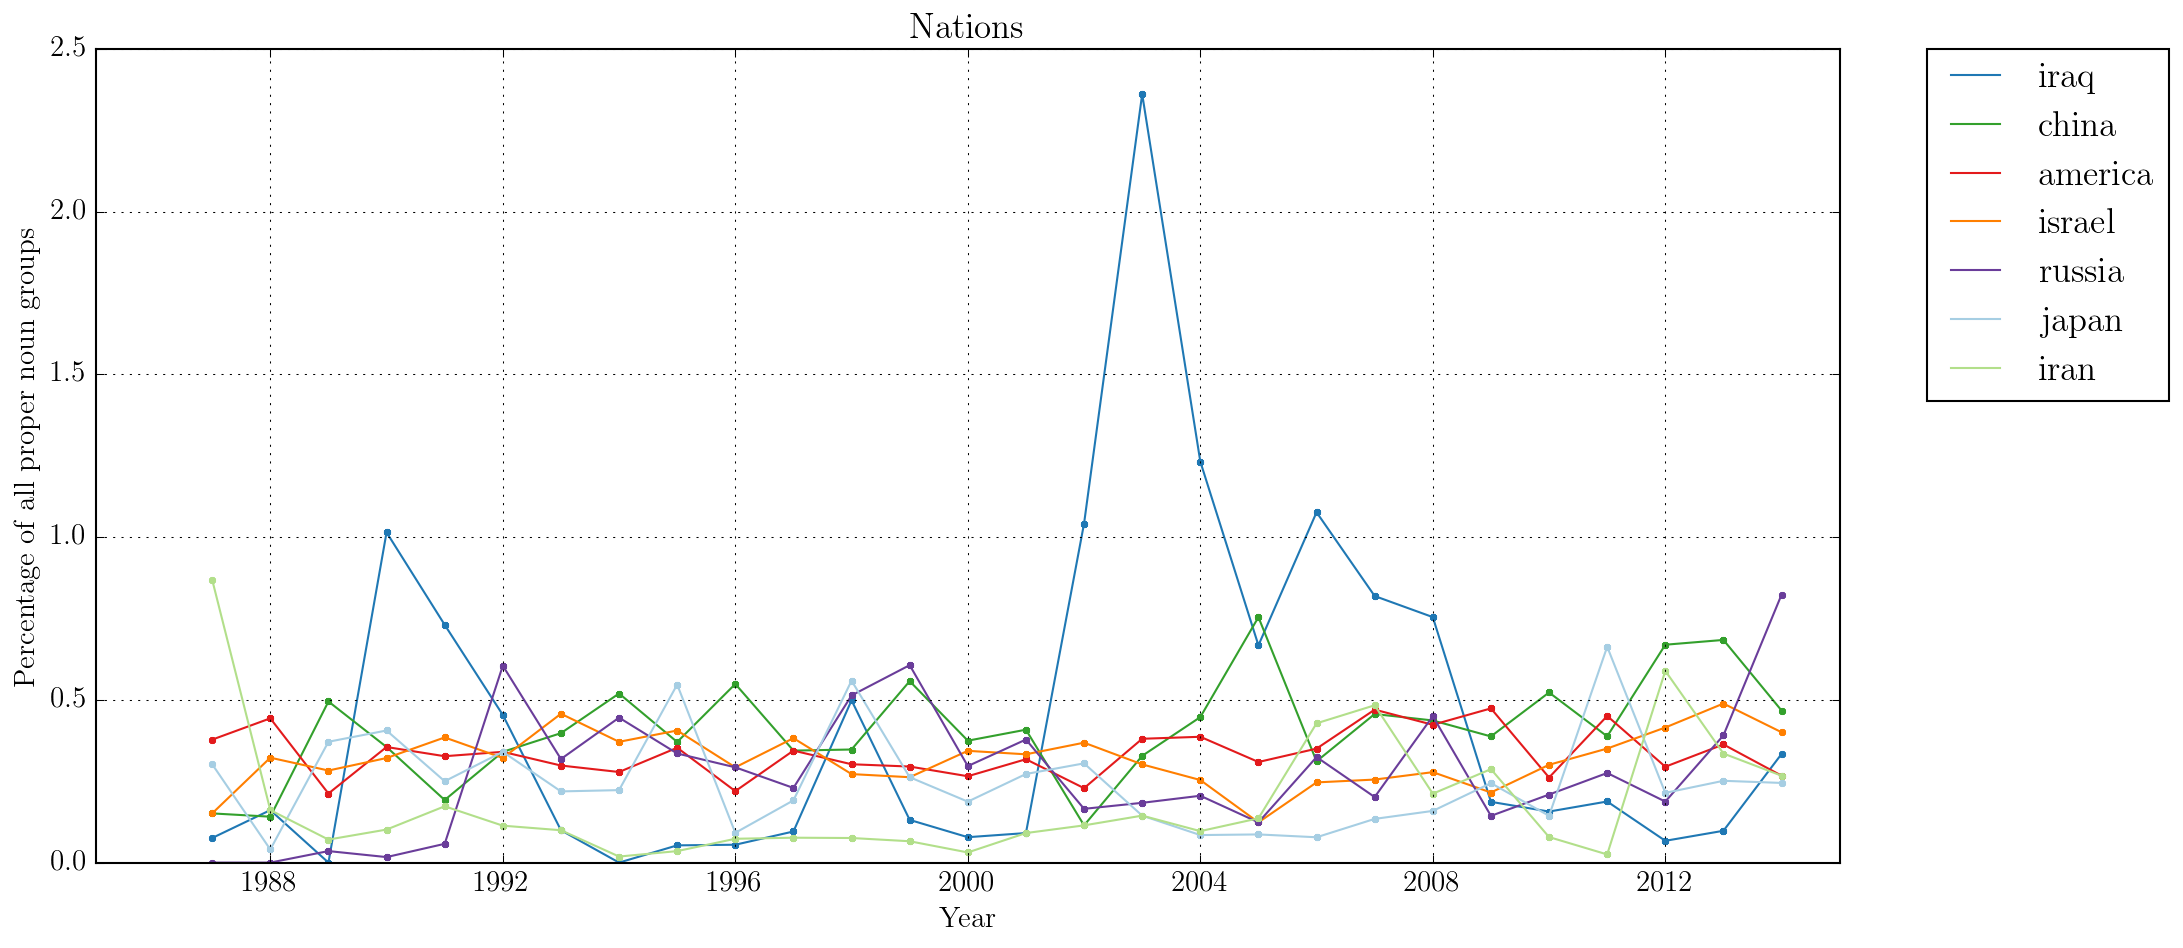
\includegraphics[width=\linewidth]{../images/nations}
                  \caption{Nations} \label{fig:b}
                  \end{subfigure}

                  \medskip
                  \begin{subfigure}{.64\textwidth}
                  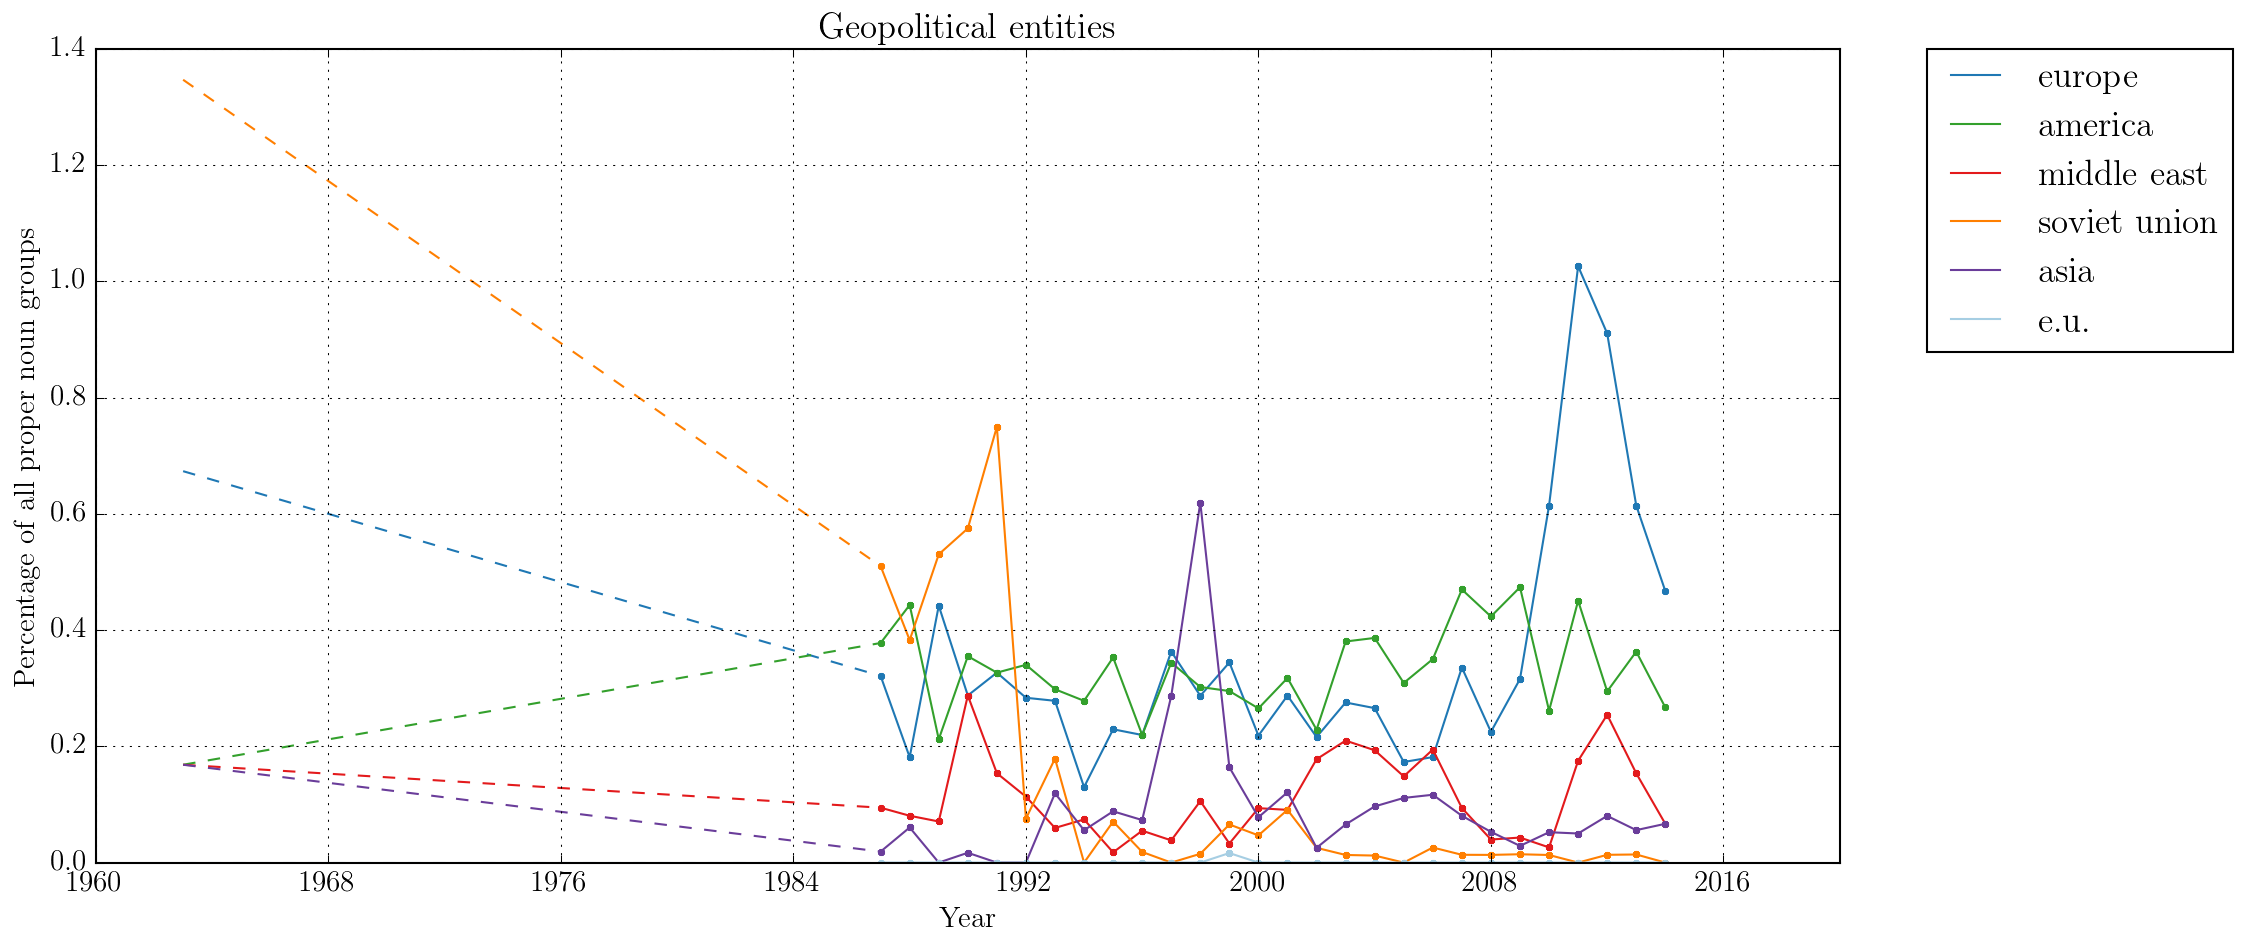
\includegraphics[width=\linewidth]{../images/geopolitical_entities}
                  \caption{Geopolitical entities} \label{fig:c}
                  \end{subfigure}
                  \begin{subfigure}{.64\textwidth}
                  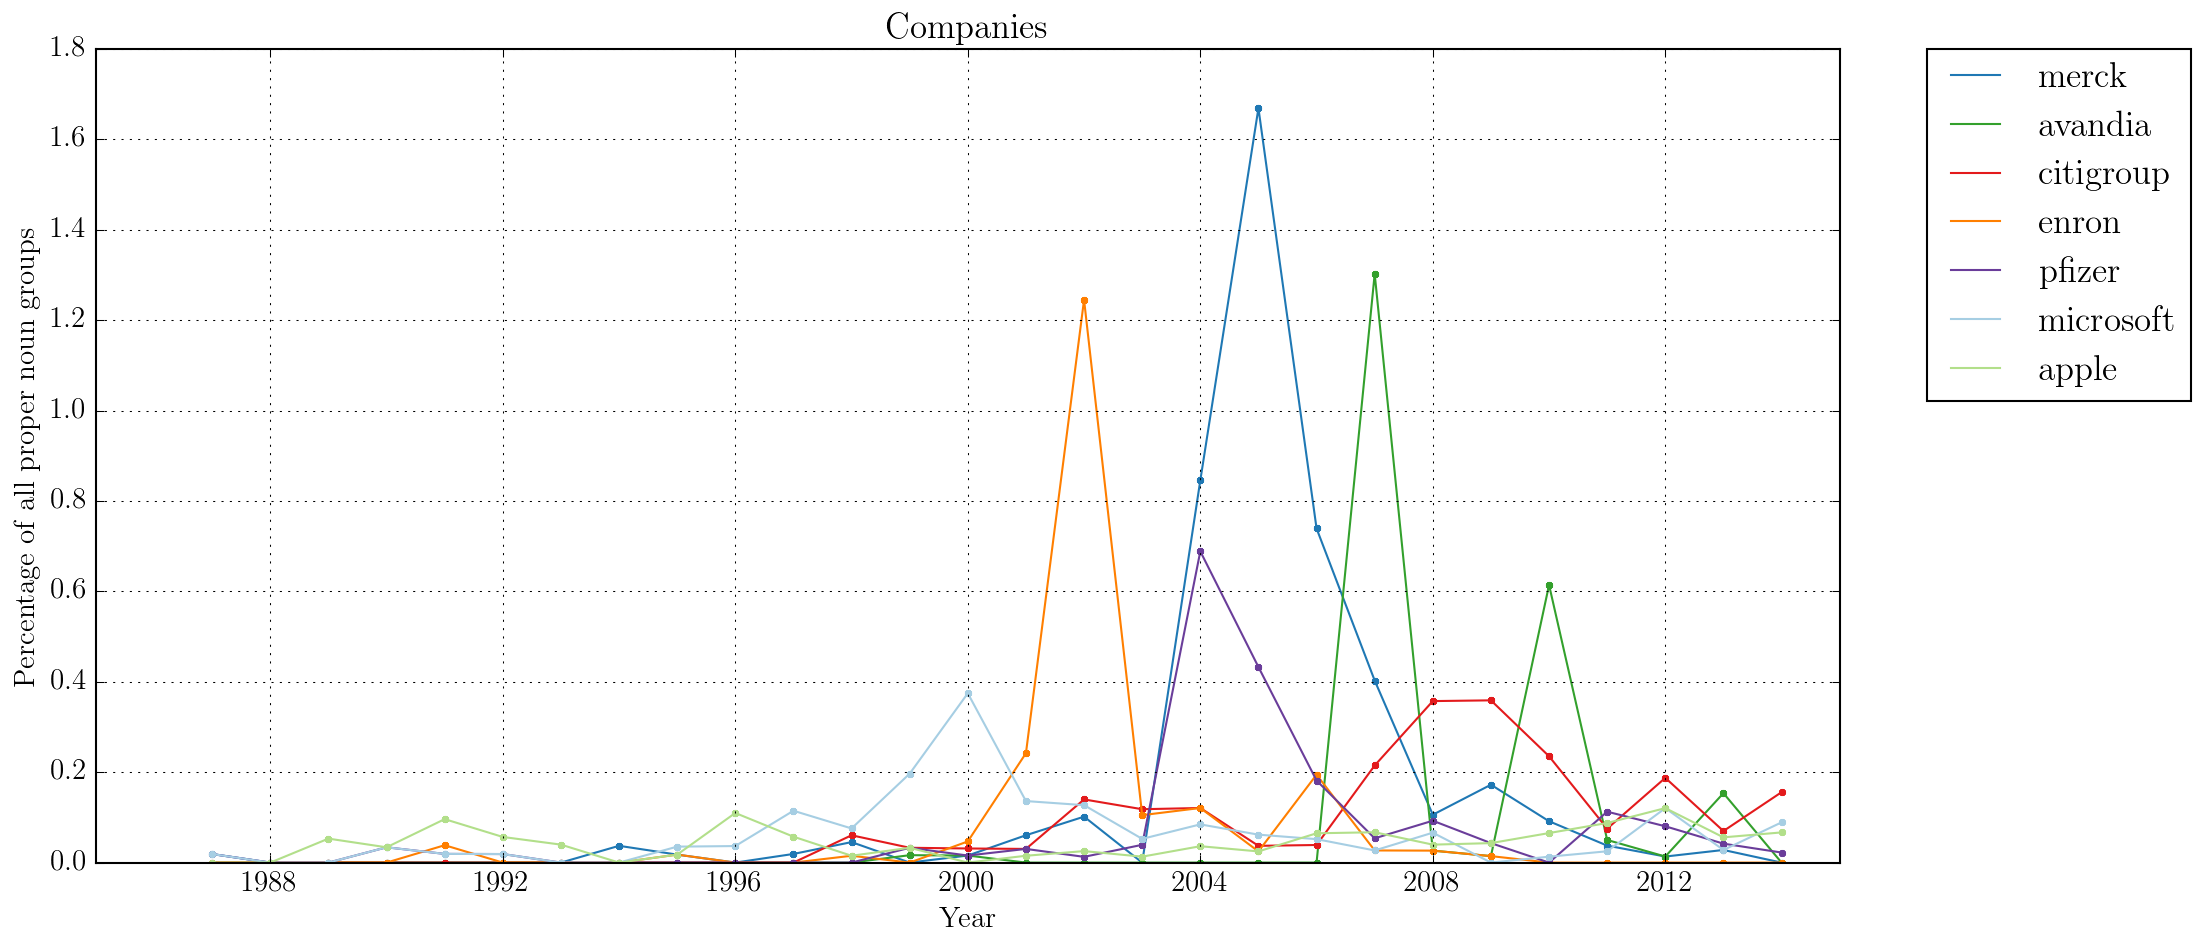
\includegraphics[width=\linewidth]{../images/companies}
                  \caption{Companies} \label{fig:d}
                  \end{subfigure}

                  \medskip
                  \begin{subfigure}{.64\textwidth}
                  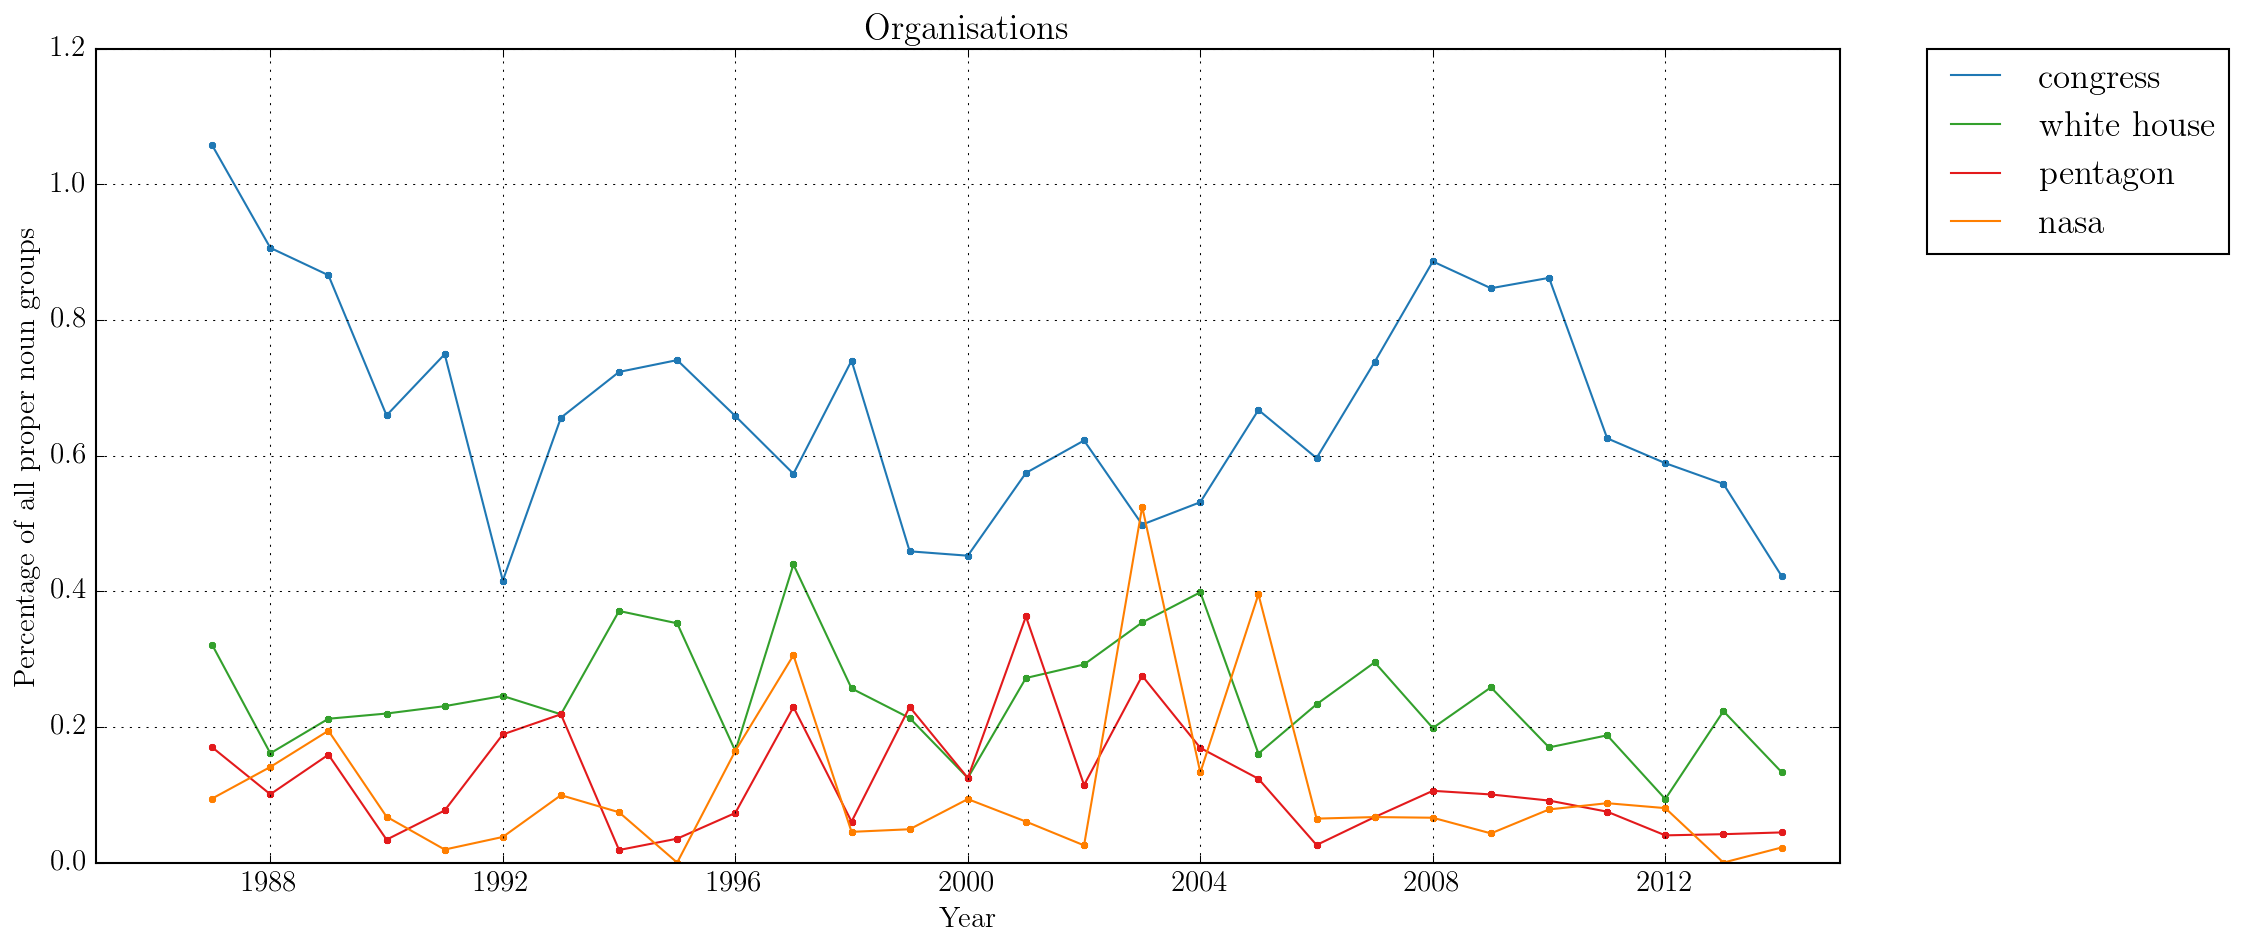
\includegraphics[width=\linewidth]{../images/organisations}
                  \caption{Organisations} \label{fig:e}
                  \end{subfigure}
                  \begin{subfigure}{.64\textwidth}
                  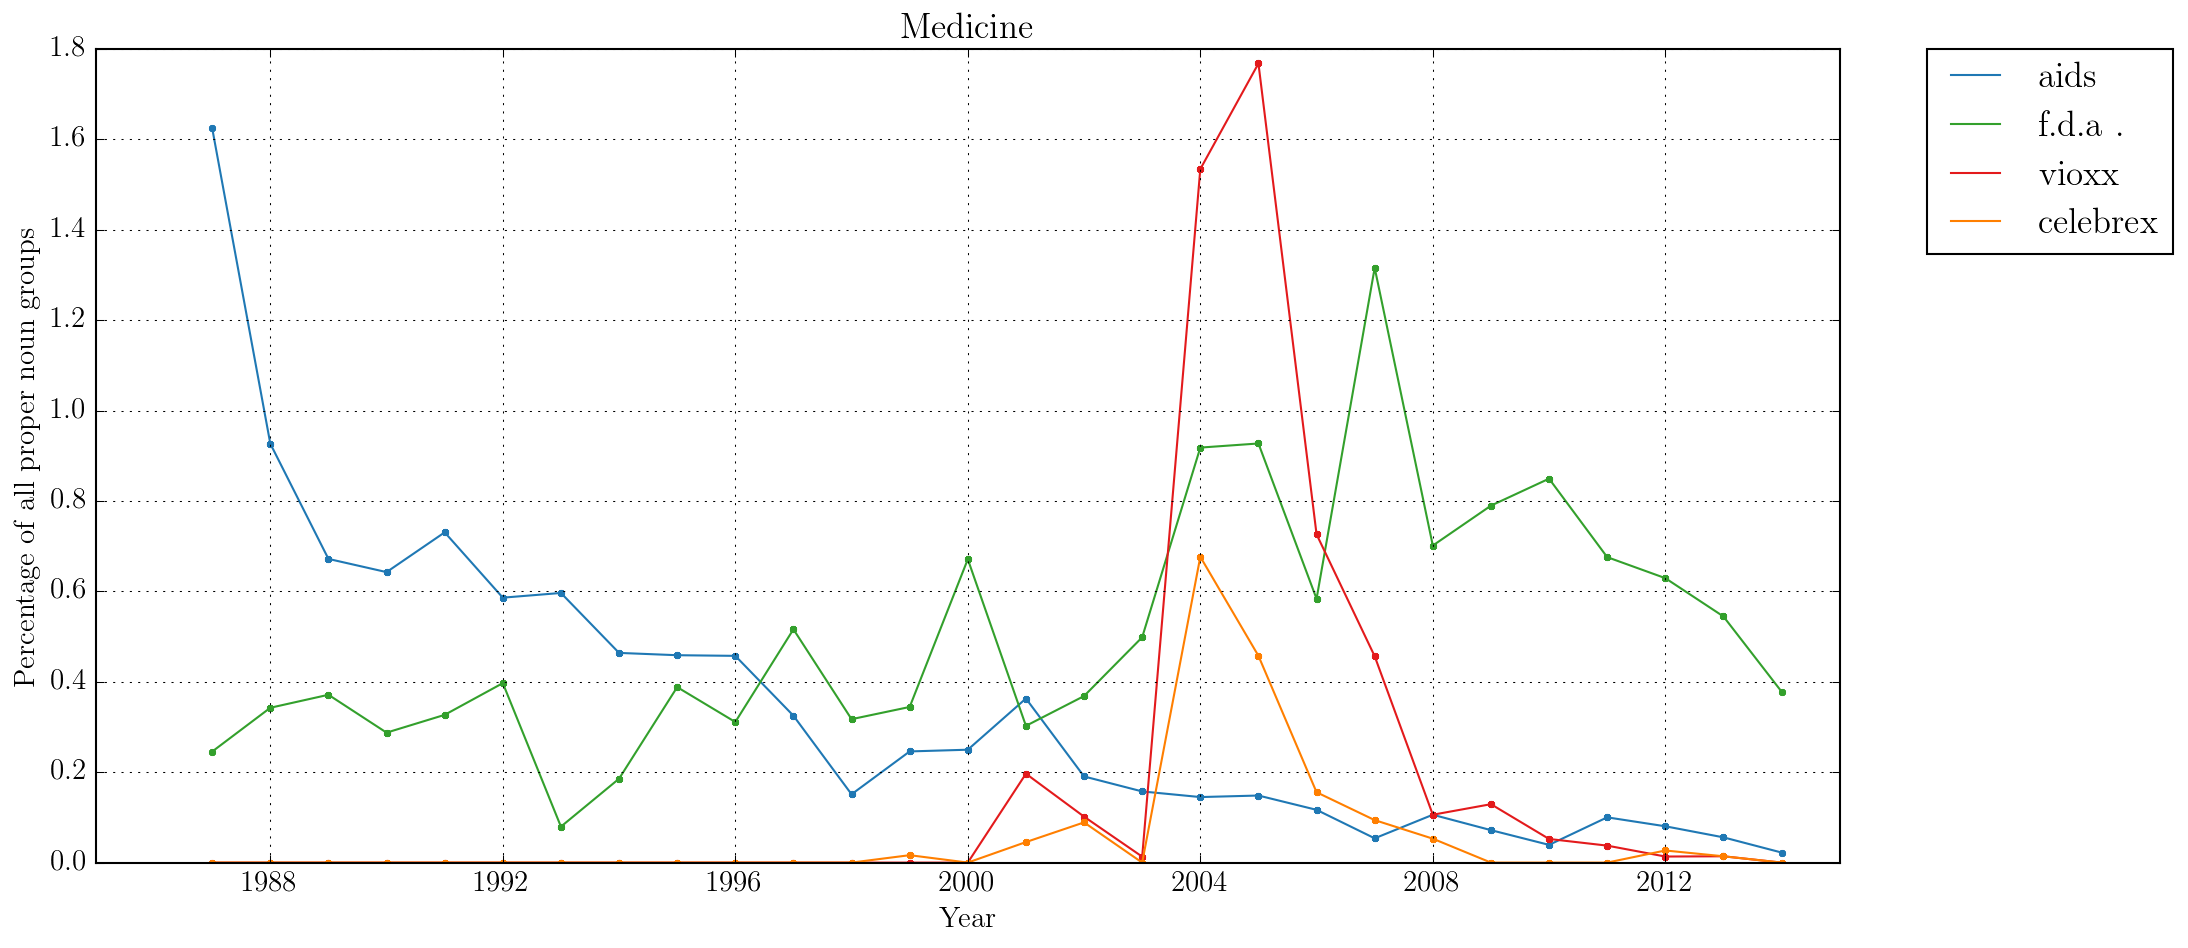
\includegraphics[width=\linewidth]{../images/medicine}
                  \caption{Medical terms} \label{fig:f}
                  \end{subfigure}
                  \caption{Proper noun groups co-occurring with risk} \label{fig:propernouns}
                  \end{figure}
                  \end{landscape}

                A number of historical events were easily recognisable within the peaks and troughs of these charts. Key events represented through these interrogations include:

                \begin{enumerate} \setlength\itemsep{0em}
                    \item US presidents and presidential candidates\endnote{Though the filtering out of titles and given names collapses the distinction between Bushes and Clintons, we can still reasonably infer which was being spoken about at which, and doubt can be eliminated by concordancing}~(Figure~\ref{fig:a})
                    \item The First Persian Gulf War (Figure~\ref{fig:b})                   
                    \item The Iraq Wars (Figure~\ref{fig:b})
                    \item September 11 and the War in Afghanistan (Figure~\ref{fig:b})   
                    \item The beginning of the 2014 Crimean crisis (Figure~\ref{fig:b})       
                    \item The Asian financial crisis (Figure~\ref{fig:c})
                    \item The breakup of the Soviet Union (Figure~\ref{fig:c})
                    \item The Eurozone crisis (Figure~\ref{fig:c})
                    \item The Space Shuttle Colombia Disaster (Figure~\ref{fig:d})
                    \item The collapse of Enron (Figure~\ref{fig:e})
                    \item The U.S. subprime mortgage crisis  (Figure~\ref{fig:e})
                    \item The U.S. outbreak of HIV and the AIDS crisis (Figure~\ref{fig:f})
                    \item The recall of Vioxx (Figure~\ref{fig:f})
                \end{enumerate}
                %
                This area of our investigation is by far the most promising as a means of connecting risk language to particular people and events. Spatial considerations have precluded a full treatment of the charting of risk language to specific events, despite the fact that enough data exists for detailed analyses of any number of potential foci. Future research that centres on detailed exploration of health domains (including the Vioxx recall) is planned.

                It should also be noted that the kinds of tasks needed for analysis of proper nouns in particular (selecting particular tokens or thematic clusters of tokens, merging results, zooming in to particular spans of time, etc.) are key components of the corpus analysis toolkit and IPython Notebook interface (\url{https://github.com/interrogator/risk}). Exploration using the purpose-built interface reveals that many topics are present in the data, but are hidden by the frequency of the very prominent examples charted here. Searching for \emph{Yugoslavia}, \emph{Bosnia}, \emph{Kosovo}, \emph{Serbia}, \emph{Mil{\u o}sevi{\'c}}, \emph{\textsc{NATO}}, (etc.), reveal expected peaks at different stages of the 1990s, despite falling outside of the range of the visualisations presented here. Given that the dataset and toolkit are open-sourced, we encourage researchers to conduct further, more specific analysis of risk language and either particular people, places and events, or risk language and topics such as health, politics, economics or sport.


%\bibliography{../references/libwin}

